%%%%%%%%%%%%%%%%%%%%%%%%%%%%%%%%%%%%%%%%%
% Short Sectioned Assignment LaTeX Template Version 1.0 (5/5/12)
% This template has been downloaded from: http://www.LaTeXTemplates.com
% Original author:  Frits Wenneker (http://www.howtotex.com)
% License: CC BY-NC-SA 3.0 (http://creativecommons.org/licenses/by-nc-sa/3.0/)
%%%%%%%%%%%%%%%%%%%%%%%%%%%%%%%%%%%%%%%%%

%----------------------------------------------------------------------------------------
%	PACKAGES AND OTHER DOCUMENT CONFIGURATIONS
%----------------------------------------------------------------------------------------

\documentclass[paper=a4, fontsize=11pt]{scrartcl} % A4 paper and 11pt font size

% ---- Entrada y salida de texto -----

\usepackage[T1]{fontenc} % Use 8-bit encoding that has 256 glyphs
\usepackage[utf8]{inputenc}
%\usepackage{fourier} % Use the Adobe Utopia font for the document - comment this line to return to the LaTeX default

% ---- Idioma --------

\usepackage[spanish, es-tabla]{babel} % Selecciona el español para palabras introducidas automáticamente, p.ej. "septiembre" en la fecha y especifica que se use la palabra Tabla en vez de Cuadro

% ---- Otros paquetes ----

\usepackage[hidelinks]{hyperref} % Estilo para los enlaces
\hypersetup{
  colorlinks   = true, %Colours links instead of ugly boxes
  urlcolor     = blue, %Colour for external hyperlinks
  linkcolor    = black, %Colour of internal links
  citecolor   = blue %Colour of citations
}
\usepackage{url} % ,href} %para incluir URLs e hipervínculos dentro del texto (aunque hay que instalar href)
\usepackage{amsmath,amsfonts,amsthm} % Math packages
%\usepackage{graphics,graphicx, floatrow} %para incluir imágenes y notas en las imágenes
\usepackage{graphics,graphicx, float} %para incluir imágenes y colocarlas
\usepackage{eurosym}

% Para hacer tablas comlejas
%\usepackage{multirow}
%\usepackage{threeparttable}

%\usepackage{sectsty} % Allows customizing section commands
%\allsectionsfont{\centering \normalfont\scshape} % Make all sections centered, the default font and small caps

\usepackage{fancyhdr} % Custom headers and footers
\pagestyle{fancyplain} % Makes all pages in the document conform to the custom headers and footers
\fancyhead{} % No page header - if you want one, create it in the same way as the footers below
\fancyfoot[L]{} % Empty left footer
\fancyfoot[C]{} % Empty center footer
\fancyfoot[R]{\thepage} % Page numbering for right footer
\renewcommand{\headrulewidth}{0pt} % Remove header underlines
\renewcommand{\footrulewidth}{0pt} % Remove footer underlines
\setlength{\headheight}{13.6pt} % Customize the height of the header

\numberwithin{equation}{section} % Number equations within sections (i.e. 1.1, 1.2, 2.1, 2.2 instead of 1, 2, 3, 4)
\numberwithin{figure}{section} % Number figures within sections (i.e. 1.1, 1.2, 2.1, 2.2 instead of 1, 2, 3, 4)
\numberwithin{table}{section} % Number tables within sections (i.e. 1.1, 1.2, 2.1, 2.2 instead of 1, 2, 3, 4)

\setlength\parindent{0pt} % Removes all indentation from paragraphs - comment this line for an assignment with lots of text

\newcommand{\horrule}[1]{\rule{\linewidth}{#1}} % Create horizontal rule command with 1 argument of height


%----------------------------------------------------------------------------------------
%	TÍTULO Y DATOS DEL ALUMNO
%----------------------------------------------------------------------------------------

\title{	
\normalfont \normalsize 
\textsc{\textbf{Ingeniería de Servidores (2016-2017)} \\ Grado en Ingeniería Informática \\ Universidad de Granada} \\ [25pt] % Your university, school and/or department name(s)
\horrule{0.5pt} \\[0.4cm] % Thin top horizontal rule
\huge Memoria Práctica 3 \\ % The assignment title
\horrule{2pt} \\[0.5cm] % Thick bottom horizontal rule
}

\author{Elena María Gómez Ríos} % Nombre y apellidos

\date{\normalsize\today} % Incluye la fecha actual

%----------------------------------------------------------------------------------------
% DOCUMENTO
%----------------------------------------------------------------------------------------

\begin{document}

\maketitle % Muestra el Título

\newpage %inserta un salto de página

\tableofcontents % para generar el índice de contenidos

\listoffigures

\listoftables

\newpage

%\textbf{NOTA: en caso de problema al compilar, compruebe que tiene el paquete: texlive-babel-spanish.noarch }  \\
 


\newpage

%----------------------------------------------------------------------------------------
%	Cuestión 1
%----------------------------------------------------------------------------------------

\section{Cuestión 1:}

\subsection{a) ¿Qué archivo le permite ver qué programas se han instalado con el gestor de paquetes?}

En Ubuntu, tal y como se explica en \cite{logApt}, en la carpeta \texttt{/var/log/apt/} hay un historial de los programas que se han instalado con el gestor de paquetes. El archivo \texttt{/var/log/apt/history.log} contiene los paquetes instalados, actualizados o desinstalados desde el inicio del mes hasta el día actual.\\
En CentOS se encuentra en \texttt{/var/log/yum.log}.

\subsection{b) ¿Qué significan las terminaciones .1.gz o .2.gz de los archivos en ese directorio?}
Las terminaciones .1.gz o .2.gz hacen referencia a archivos history.log antiguos. Tal y como se indica en \cite{logApt} ``el número de archivos history.log y el periodo de datos almacenados dependerá de la configuración de nuestra política de logs. Podemos cambiar nuestra política de logs modificando el contenido del archivo \texttt{/etc/logrotate.d/apt}.''


%----------------------------------------------------------------------------------------
%	Cuestión opcional 1
%----------------------------------------------------------------------------------------

%\section{Cuestión opcional 1:}

%\subsection{Indique qué comandos ha utilizado para realizarlo así como capturas %de pantalla del proceso de reconstrucción del RAID.}


%----------------------------------------------------------------------------------------
%	Cuestión 2
%----------------------------------------------------------------------------------------

\section{Cuestión 2:}

\subsection{¿qué archivo ha de modificar para programar una tarea? Escriba la línea necesaria para ejecutar una vez al día una copia del directorio $\sim$/codigo a $\sim$/seguridad/\$fecha donde \$fecha es la fecha actual (puede usar el comando date).}

Tal y como se vio en las prácticas de la asignatura de Sistemas Operativos hay que modificar el archivo de configuración del \texttt{cron}, que se encuentra en \texttt{/etc/crontab}. Pero dicha modificación no debe hacerse directamente en éste archivo, si no que se debe utilizar el comando \texttt{crontab -e} por seguridad.\\
El formato del archivo crontab es el siguiente:\\
\texttt{minuto \hspace{0.5cm} hora  \hspace{0.5cm} día-del-mes \hspace{0.5cm} mes \hspace{0.5cm} día-de-la-semana  \hspace{0.5cm} orden}\\
Los valores permitidos para minuto son 0-59, para hora 0-23, para día-del-mes 1-31, para mes 1-12 y para día-de-la-semana 0-7. En todos los casos un * indica cualquier valor posible. Por lo tanto la línea que se debe añadir para que se ejecute una vez al día es:\\
\texttt{0 \hspace{0.5cm} 0 \hspace{0.5cm} * \hspace{0.5cm} * \hspace{0.5cm} * \hspace{0.5cm} ./script\_cron.sh}\\
Siendo el contenido del script el que se muestra en la figura \ref{fig:ejercicio2-1}. Para probarlo he cambiado la hora de ejecución para que se ejecute cada minuto y compruebo que crea la carpeta de forma correcta \ref{fig:ejercicio2_2}.

\begin{figure}[H] 
	\centering
	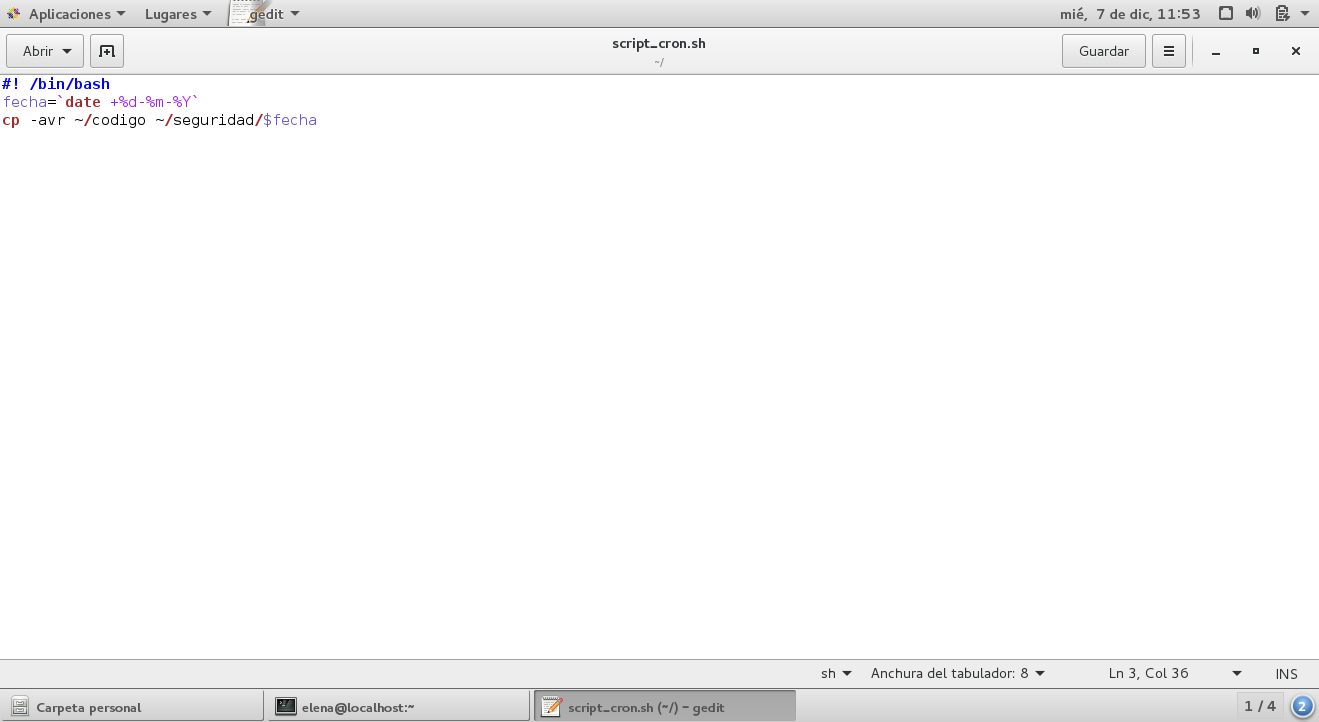
\includegraphics[width=14.7cm]{./img/ejercicio2-1.png} 	
	\caption{CentOS, crear script para crontab.} \label{fig:ejercicio2-1}
\end{figure}

\begin{figure}[H] 
	\centering
	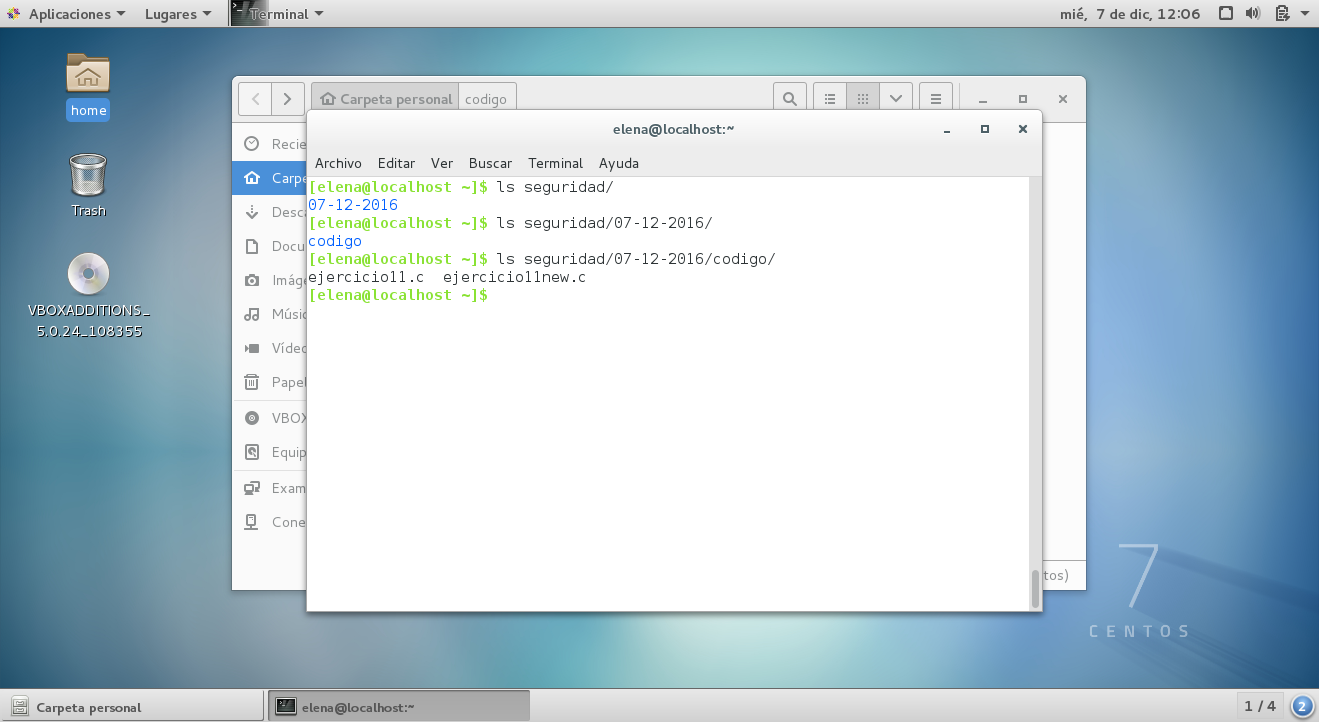
\includegraphics[width=14.7cm]{./img/ejercicio2_2.png} 	
	\caption{CentOS, comprobación del correcto funcionamiento de cron.} \label{fig:ejercicio2_2}
\end{figure}



%----------------------------------------------------------------------------------------
%	Cuestión 3
%----------------------------------------------------------------------------------------

\section{Cuestión 3:}

\subsection{Pruebe a ejecutar el comando, conectar un dispositivo USB y vuelva a ejecutar el comando. Copie y pegue la salida del comando. (considere usar dmesg | tail). Comente qué observa en la información mostrada.}

En la figura \ref{fig:ejercicio3} se muestra en primer lugar que aún no se ha conectado el USB, luego se conecta un dispositivo USB y se muestran datos sobre dicho dispositivo. Finalmente se desconecta el USB y se muestra que está desconectado.

\begin{figure}[H] 
	\centering
	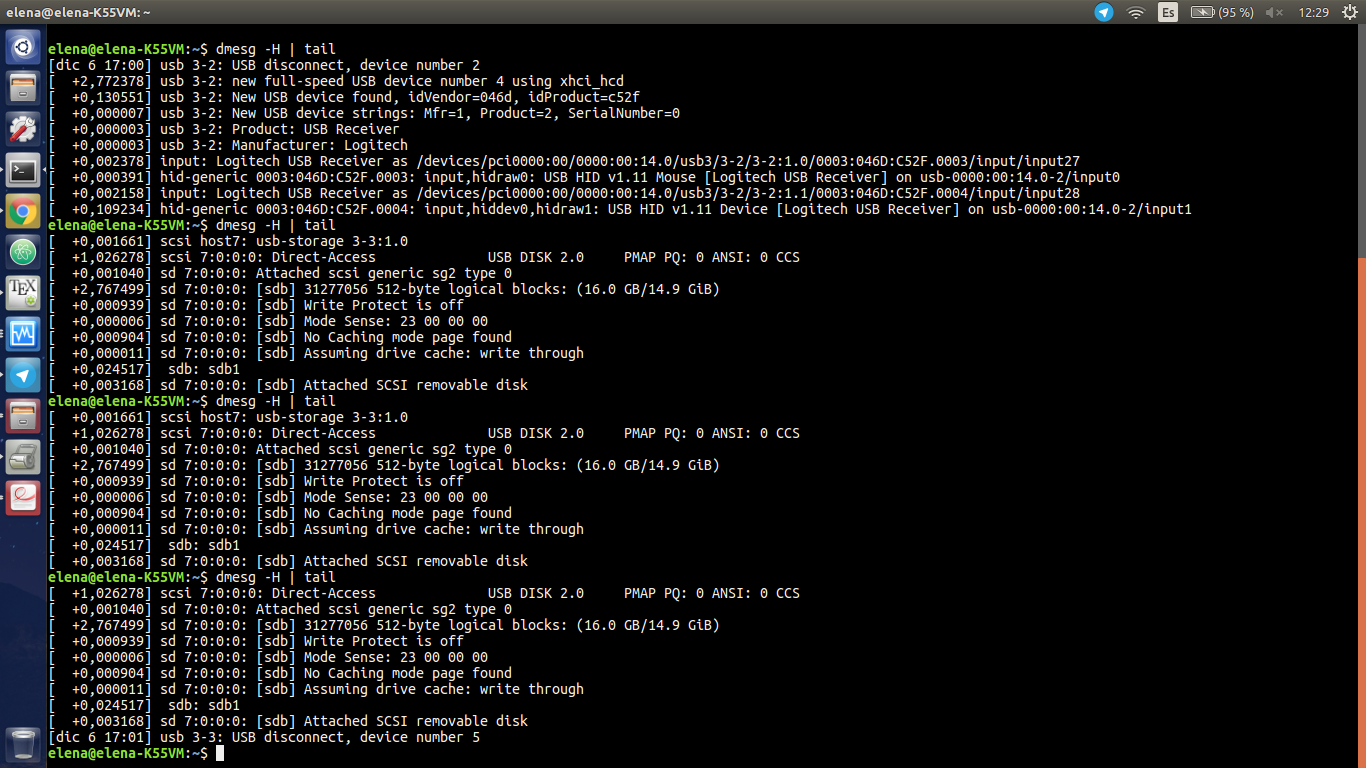
\includegraphics[width=14.7cm]{./img/ejercicio3.png} 	
	\caption{Ubuntu, comando dmesg.} \label{fig:ejercicio3}
\end{figure}


%----------------------------------------------------------------------------------------
%	Cuestión 4
%----------------------------------------------------------------------------------------

\section{Cuestión 4:}

\subsection{Ejecute el monitor de ``System Performance'' y muestre el resultado. Incluya capturas de pantalla comentando la información que  aparece.}

Para ejecutar el monitor ``System Performance'', en el panel de la izquierda, debemos ir a la carpeta ``Conjunto de recopiladores de datos'' y dentro de ésta desplegamos la carpeta ``Sistema'', donde nos aparecerá el monitor.

Los resultados se guardan dentro de la carpeta ``Informes''. Vamos a comentar una serie de apartados de todos los posibles. En la figura \ref{fig:ejercicio4_1} se muestra la información de rendimiento del sistema, un resumen y los resultados del diagnóstico, donde por ejemplo se puede observar que el uso de la memoria es del 44\% en reposo.

En las figuras \ref{fig:ejercicio4_2} y \ref{fig:ejercicio4_3} podemos observar las estadísticas del informe, donde aparece la información del equipo, archivos y eventos procesados.

En la figura \ref{fig:ejercicio4_4} se muestra la memoria utilizada por cada proceso que estaba en funcionamiento durante la monitorización, por ejemplo el proceso \texttt{powershell}.

En la figura \ref{fig:ejercicio4_5} aparece la información general del sistema, como el \% de cuota de Registro en uso o los cambios de contexto, entre otros.

\begin{figure}[H] 
	\centering
	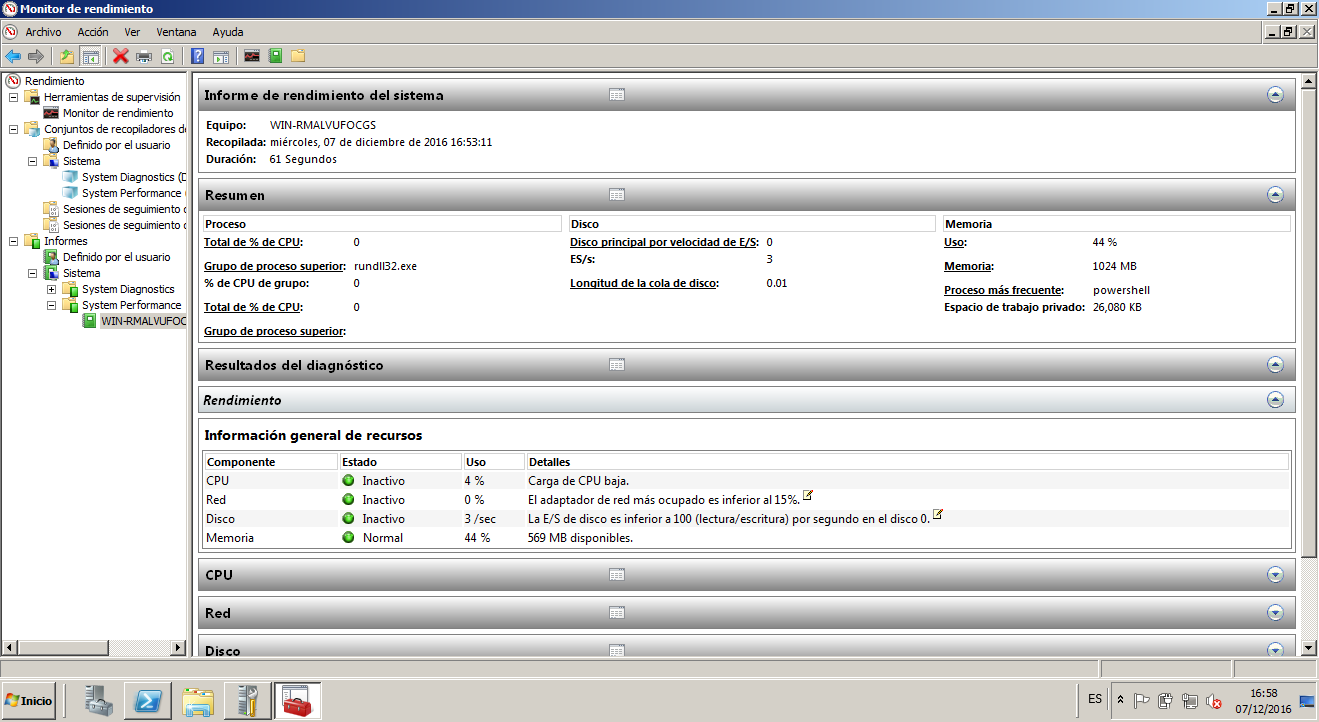
\includegraphics[width=14.7cm]{./img/ejercicio4_1.png} 	
	\caption{Windows, monitor de rendimiento, informe.} \label{fig:ejercicio4_1}
\end{figure}

\begin{figure}[H] 
	\centering
	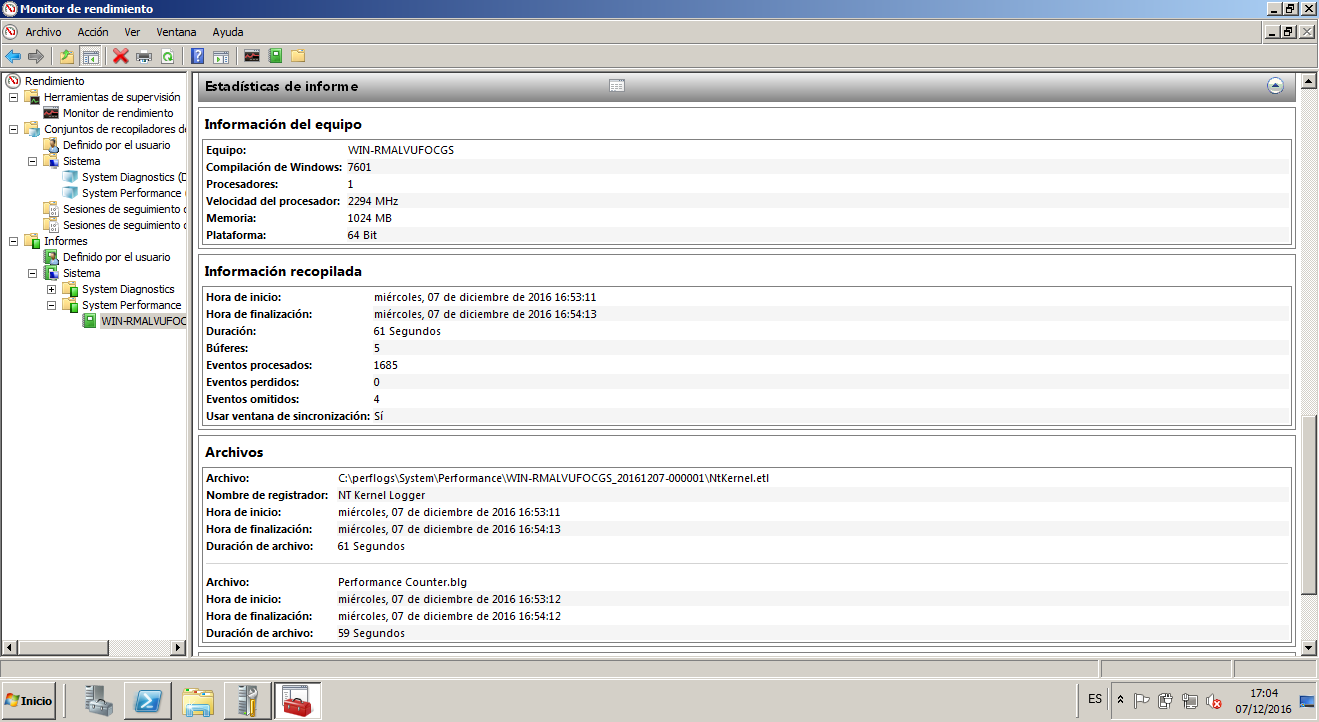
\includegraphics[width=14.7cm]{./img/ejercicio4_2.png} 	
	\caption{Windows, monitor de rendimiento, estadísticas I.} \label{fig:ejercicio4_2}
\end{figure}

\begin{figure}[H] 
	\centering
	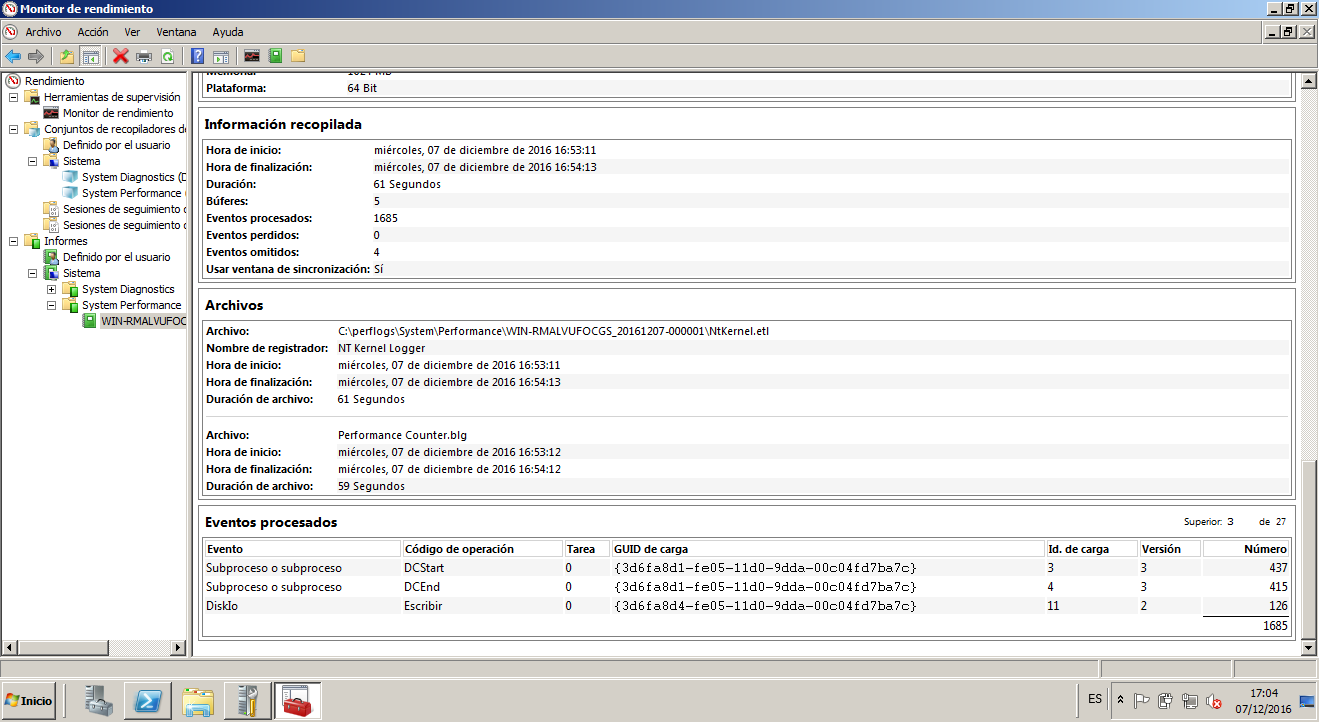
\includegraphics[width=14.7cm]{./img/ejercicio4_3.png} 	
	\caption{Windows, monitor de rendimiento, estadísticas II} \label{fig:ejercicio4_3}
\end{figure}

\begin{figure}[H] 
	\centering
	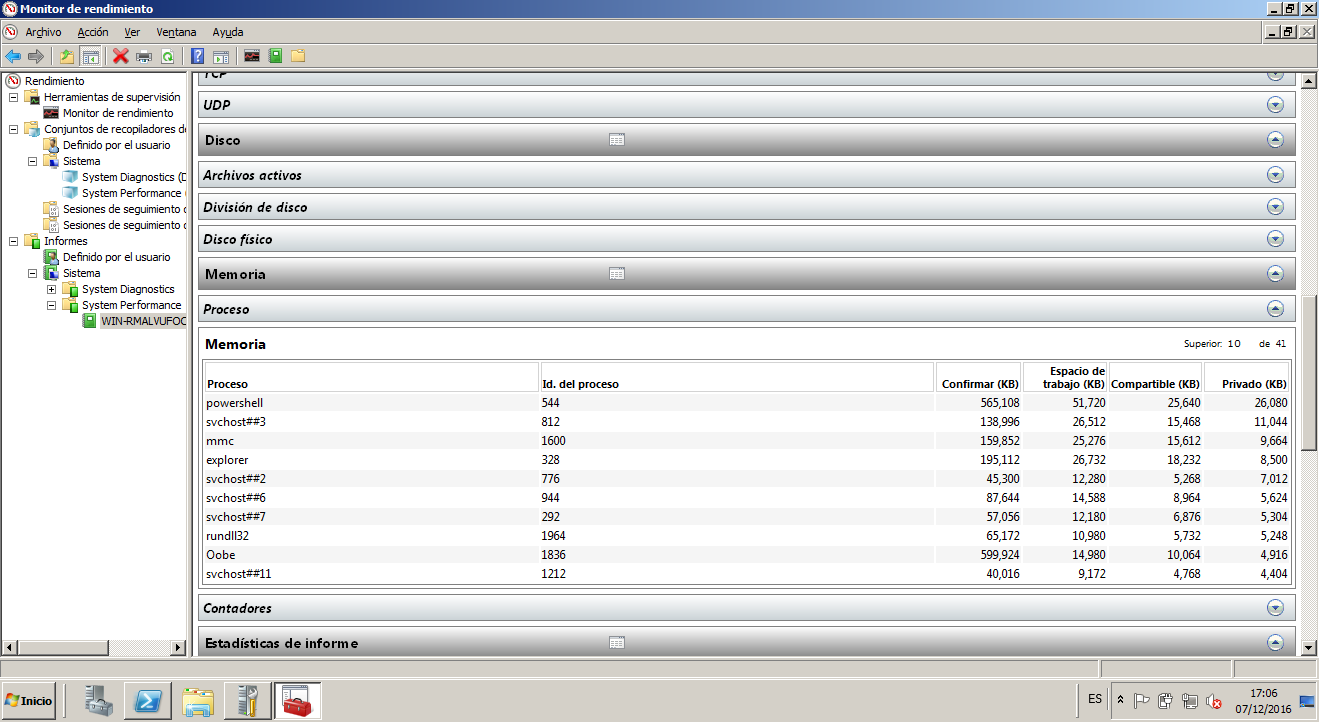
\includegraphics[width=14.7cm]{./img/ejercicio4_4.png} 	
	\caption{Windows, monitor de rendimiento, memoria.} \label{fig:ejercicio4_4}
\end{figure}

\begin{figure}[H] 
	\centering
	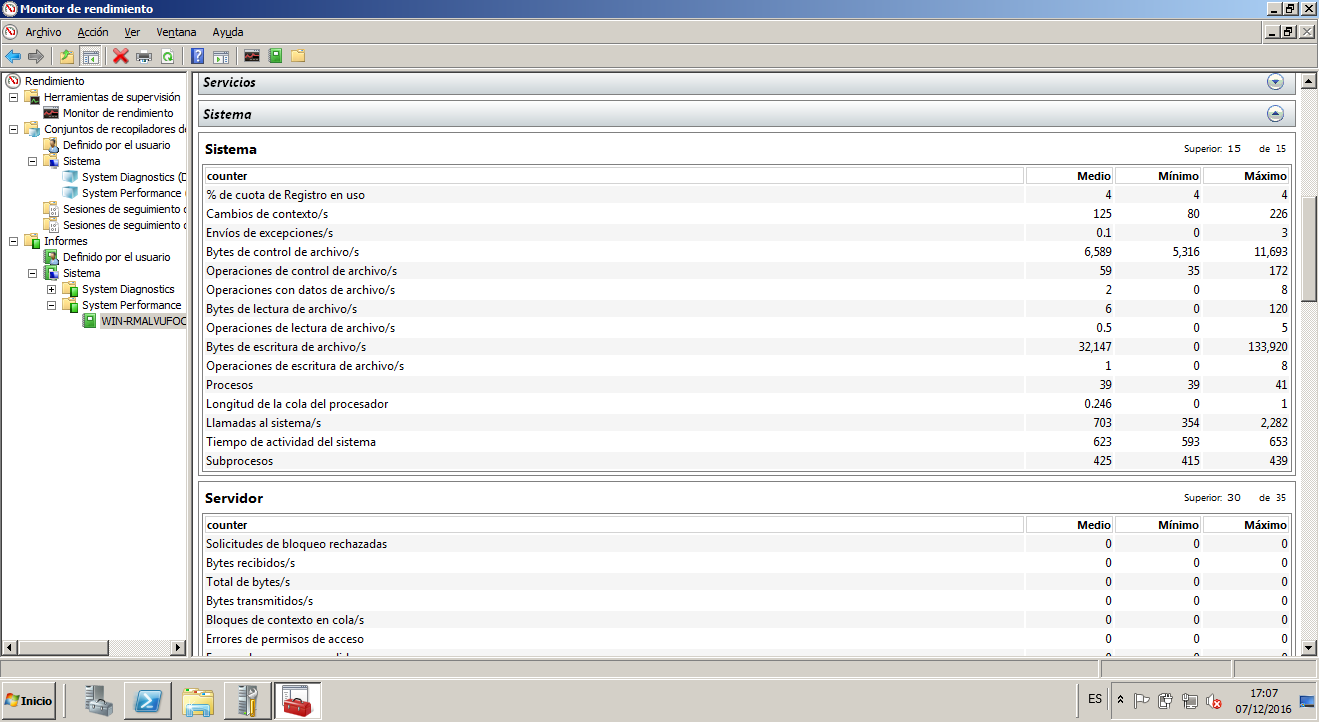
\includegraphics[width=14.7cm]{./img/ejercicio4_5.png} 	
	\caption{Windows, monitor de rendimiento, sistema.} \label{fig:ejercicio4_5}
\end{figure}



%----------------------------------------------------------------------------------------
%	Cuestión 5
%----------------------------------------------------------------------------------------

\section{Cuestión 5:}
\subsection{Cree un recopilador de datos definido por el usuario (modo avanzado) que incluya tanto el contador de rendimiento como los datos de seguimiento:}

\begin{itemize}
	\item \textbf{Todos los referentes al procesador, al proceso y al servicio web.}
	\item \textbf{Intervalo de muestra 15 segundos.}
	\item \textbf{Almacene el resultado en el directorio Escritorio\textbackslash logs.}
	\item \textbf{Incluya las capturas de pantalla de cada paso.}
\end{itemize}


Para crear un nuevo conjunto de recopiladores de datos hacemos clic derecho sobre la carpeta ``Definido por el usuario'', que está en la carpeta ``Conjuntos de recopiladores de datos'', y creamos uno nuevo tal y como se muestra en la figura \ref{fig:ejercicio5_1}, seleccionando ``crear manualmente (avanzado)''. Seleccionamos los tipos de datos que queremos incluir como se ve en la figura \ref{fig:ejercicio5_2} y continuamos. Agregamos los contadores de rendimiento que se indican (figuras \ref{fig:ejercicio5_3} y \ref{fig:ejercicio5_4}), seleccionando el intervalo de muestra en 15 segundos. Indicamos donde se van a guardar los resultados (figura \ref{fig:ejercicio5_5}) y finalizamos el proceso. Ahora nos deberá aparece el nuevo monitor como se muestra en la figura \ref{fig:ejercicio5_6}.

\begin{figure}[H] 
	\centering
	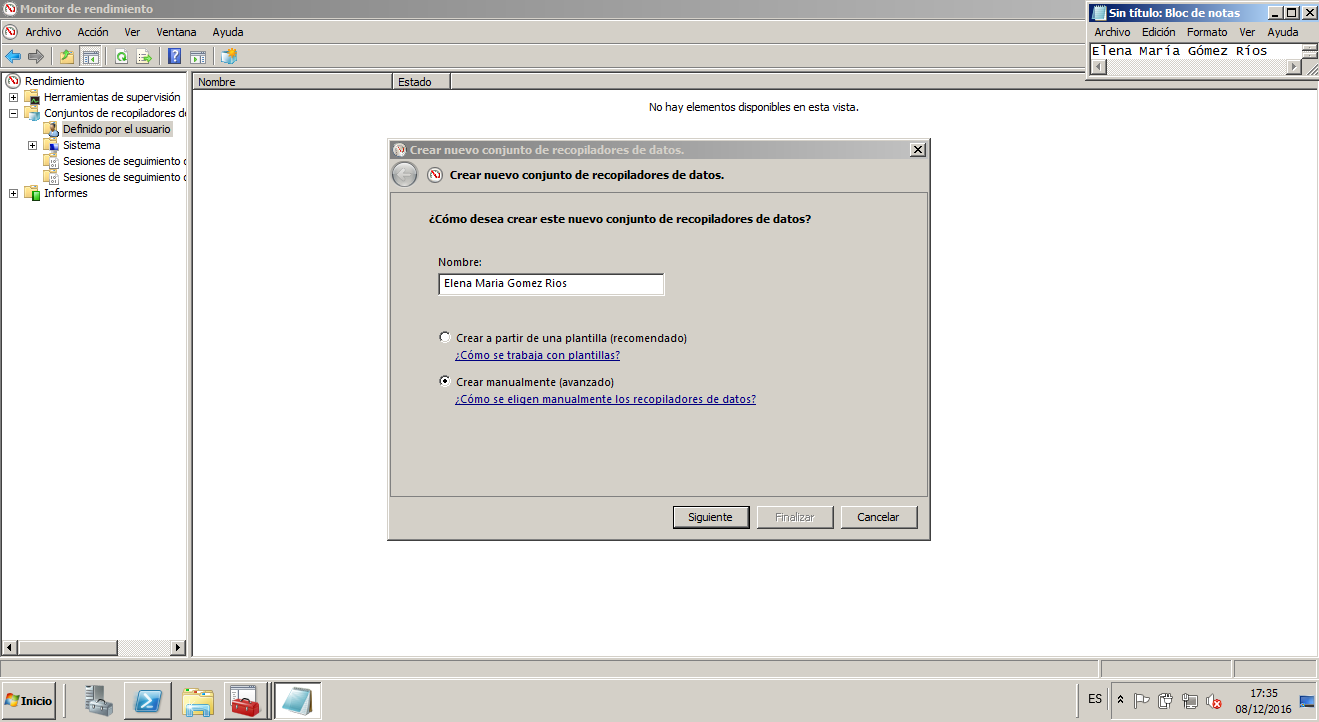
\includegraphics[width=14.7cm]{./img/ejercicio5_1.png} 	
	\caption{Windows, crear recopilador de datos I.} \label{fig:ejercicio5_1}
\end{figure}

\begin{figure}[H] 
	\centering
	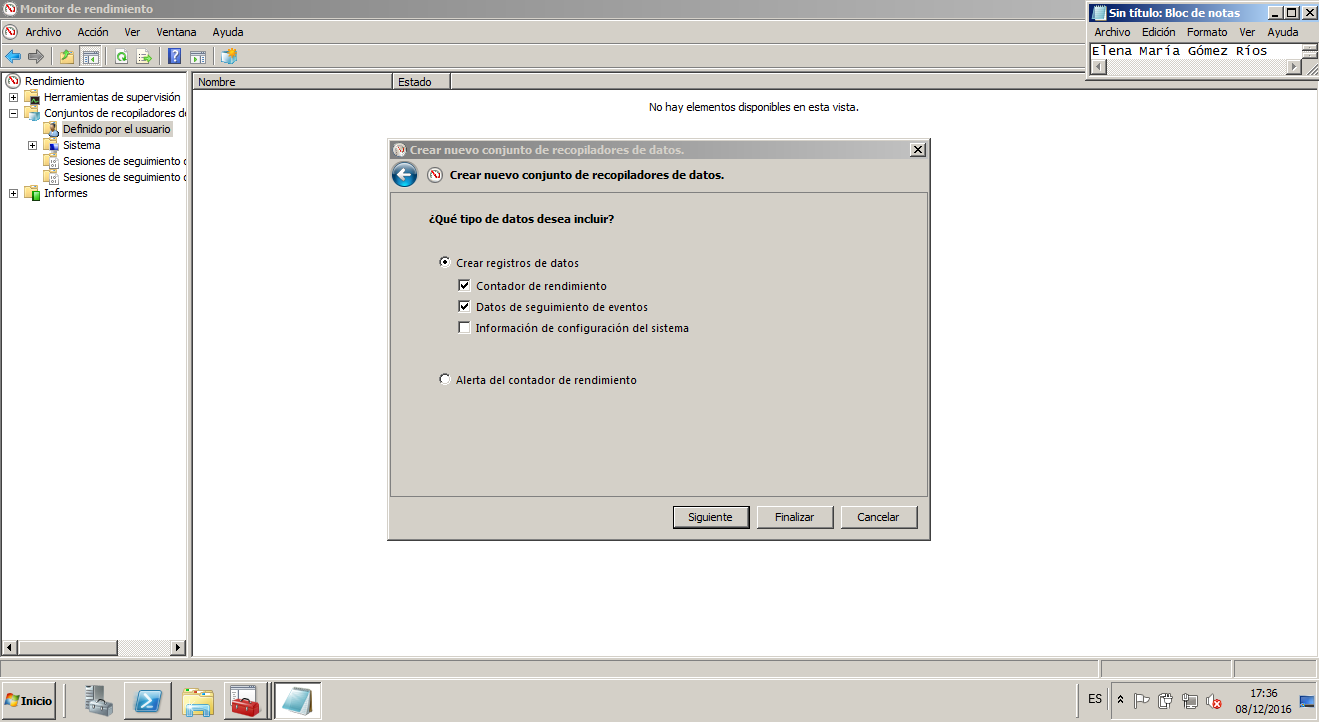
\includegraphics[width=14.7cm]{./img/ejercicio5_2.png} 	
	\caption{Windows, crear recopilador de datos II.} \label{fig:ejercicio5_2}
\end{figure}

\begin{figure}[H] 
	\centering
	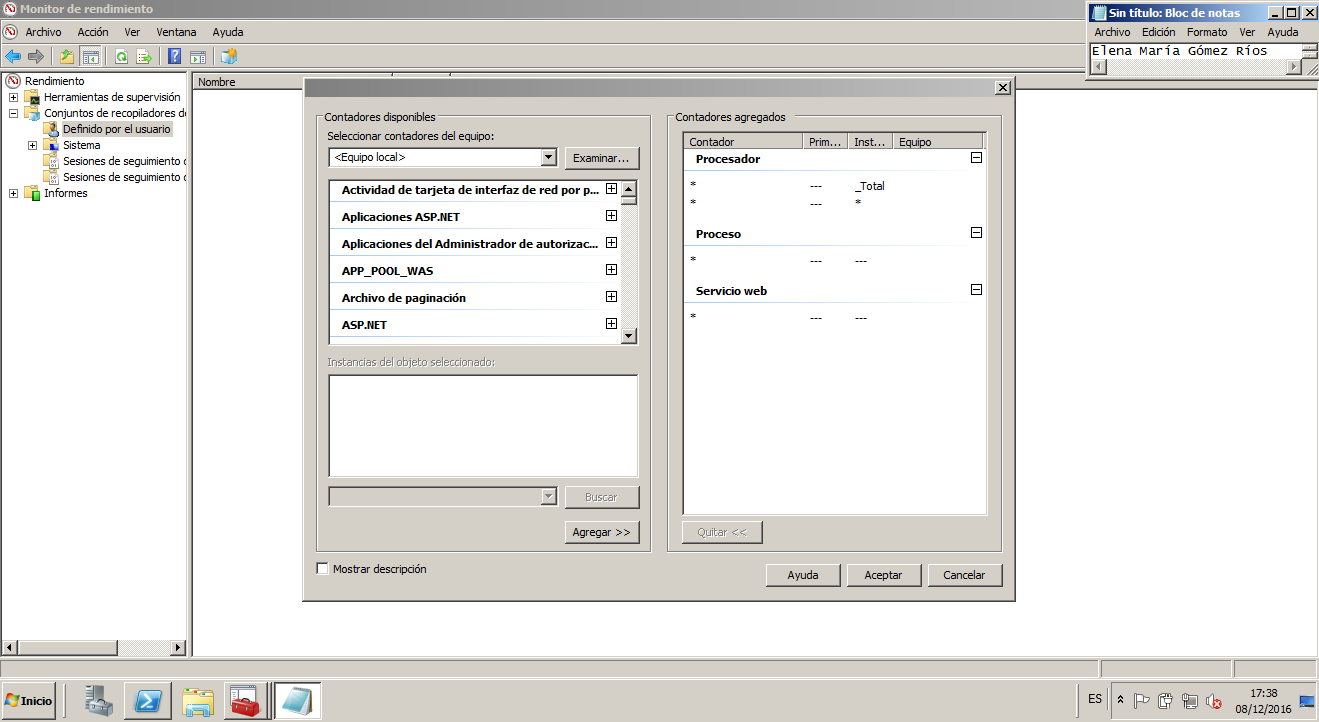
\includegraphics[width=14.7cm]{./img/ejercicio5_3.png} 	
	\caption{Windows, crear recopilador de datos III.} \label{fig:ejercicio5_3}
\end{figure}

\begin{figure}[H] 
	\centering
	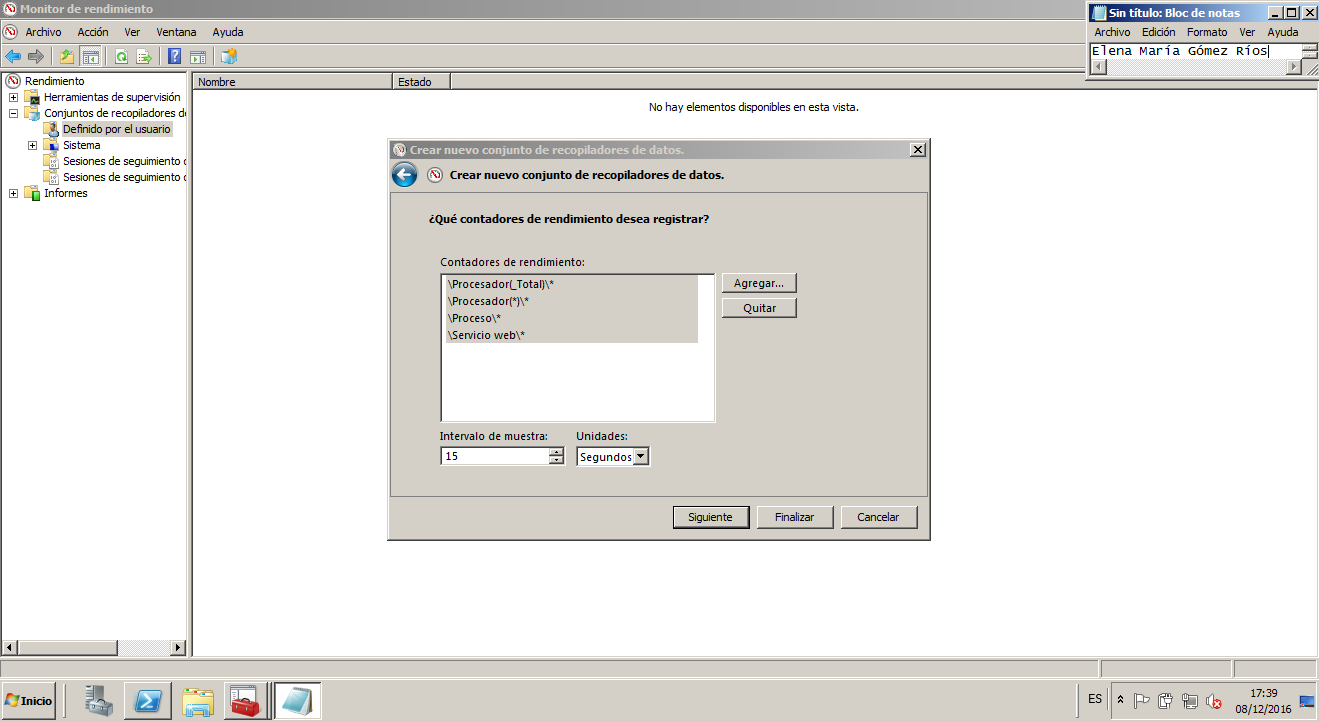
\includegraphics[width=14.7cm]{./img/ejercicio5_4.png} 	
	\caption{Windows, crear recopilador de datos IV.} \label{fig:ejercicio5_4}
\end{figure}

\begin{figure}[H] 
	\centering
	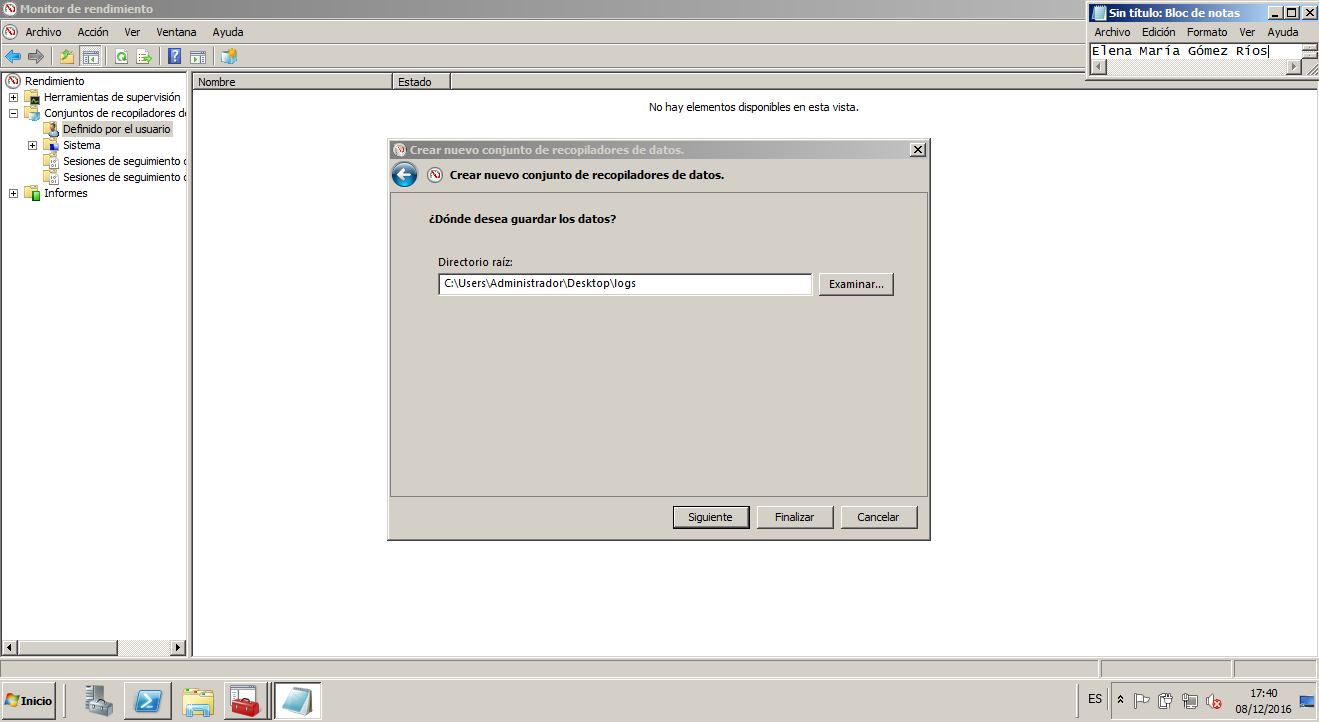
\includegraphics[width=14.7cm]{./img/ejercicio5_5.png} 	
	\caption{Windows, crear recopilador de datos V.} \label{fig:ejercicio5_5}
\end{figure}

\begin{figure}[H] 
	\centering
	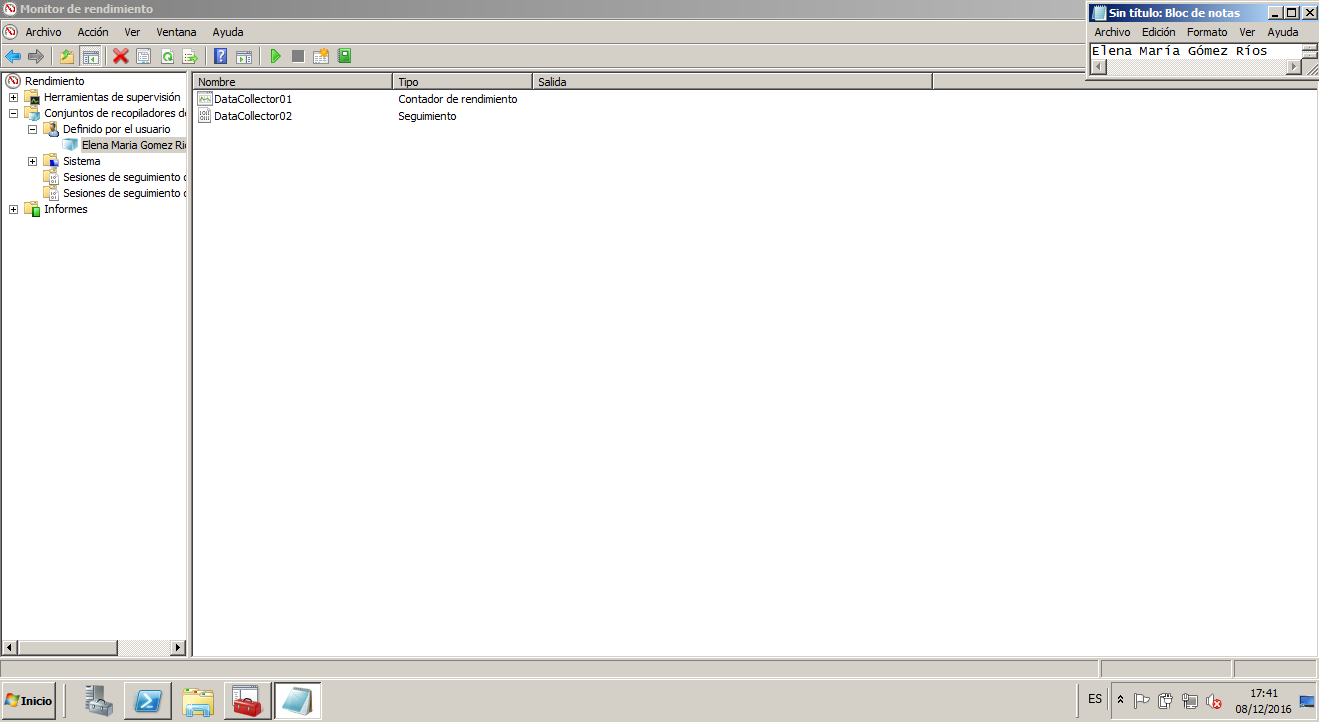
\includegraphics[width=14.7cm]{./img/ejercicio5_6.png} 	
	\caption{Windows, crear recopilador de datos VI.} \label{fig:ejercicio5_6}
\end{figure}


%----------------------------------------------------------------------------------------
%	Cuestión 6
%----------------------------------------------------------------------------------------
\section{Cuestión 6:}
 
\subsection{Visite la web del proyecto y acceda a la demo que proporcionan (http://demo.munin-monitoring.org/) donde se muestra cómo monitorizan un servidor. Monitorice varios parámetros y haga capturas de pantalla de lo que está mostrando comentando qué observa.}

Con la demo de munin se pueden monitorizar muchos parámetros, vamos a comentar algunos de ellos.

\begin{itemize}
	\item Monitorización de las CPUs (figura \ref{fig:ejercicio6_1}). En esta gráfica el intervalo de tiempo de la monitorización es semanal, se analizan cuatro CPUs. Se puede apreciar un aumento de trabajo a partir del lunes en cada una de las CPUs.
	\item Monitorización de la caché (figura \ref{fig:ejercicio6_2}). El intervalo de tiempo de esta gráfica es diario, se puede observar que es prácticamente estable a excepción del jueves entre las 6:00 y las 12:00 donde hay una mayor carga del buffer.
	\item Monitorización de la red (figura \ref{fig:ejercicio6_3}). En la gráfica se indica que a partir del lunes se produce un aumento del tráfico de la red aunque anteriormente haya picos esporádicos. Según parece a última hora del miércoles empieza a estabilizarse en sus valores anteriores. 
	\item Monitorización del uso de la CPU (figura \ref{fig:ejercicio6_4}). Como se puede observar en la gráfica prácticamente todo el tiempo se está ejecutando el proceso \texttt{idle}, que es aquel que se ejecuta cuando el procesador no tiene ninguna tarea que hacer. Aunque como es lógico el usuario y el sistema también realizan pequeñas tareas que no suponen prácticamente nada para la CPU.
\end{itemize}

\begin{figure}[H] 
	\centering
	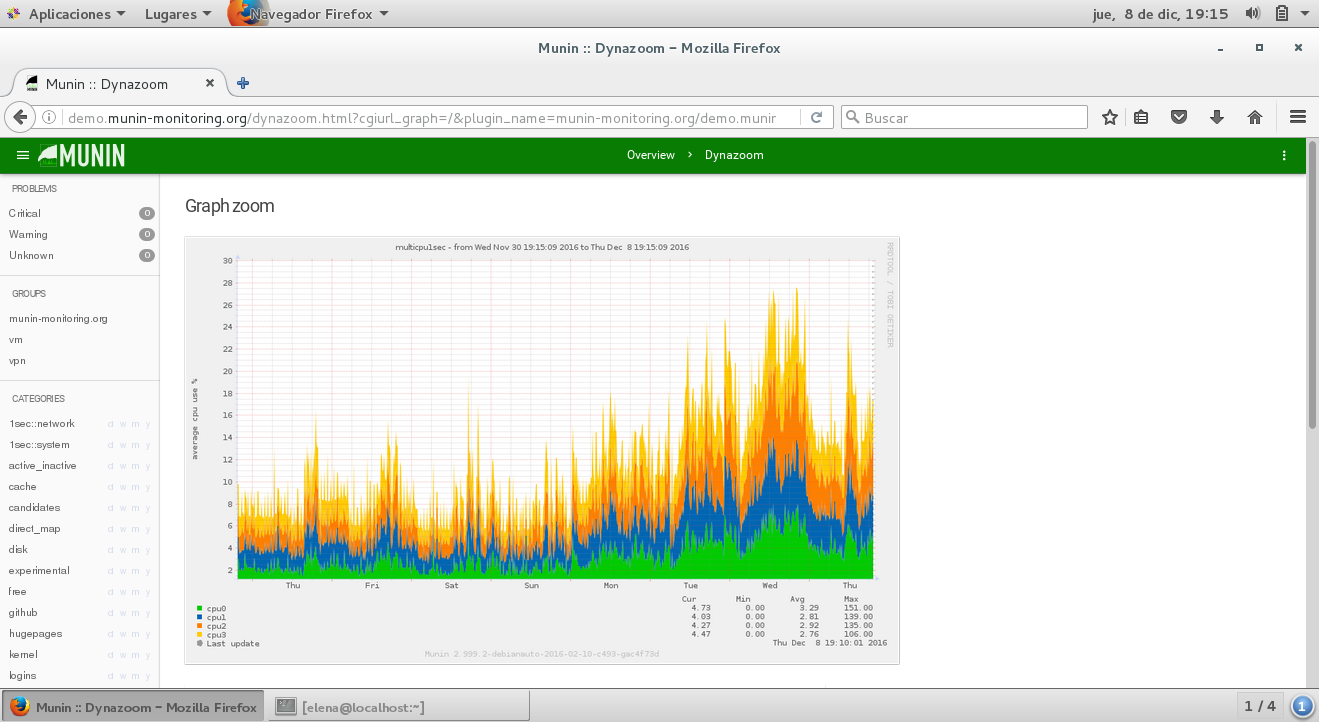
\includegraphics[width=14.7cm]{./img/ejercicio6_1.png} 	
	\caption{Demo munin, monitorización de las CPUs.} \label{fig:ejercicio6_1}
\end{figure}

\begin{figure}[H] 
	\centering
	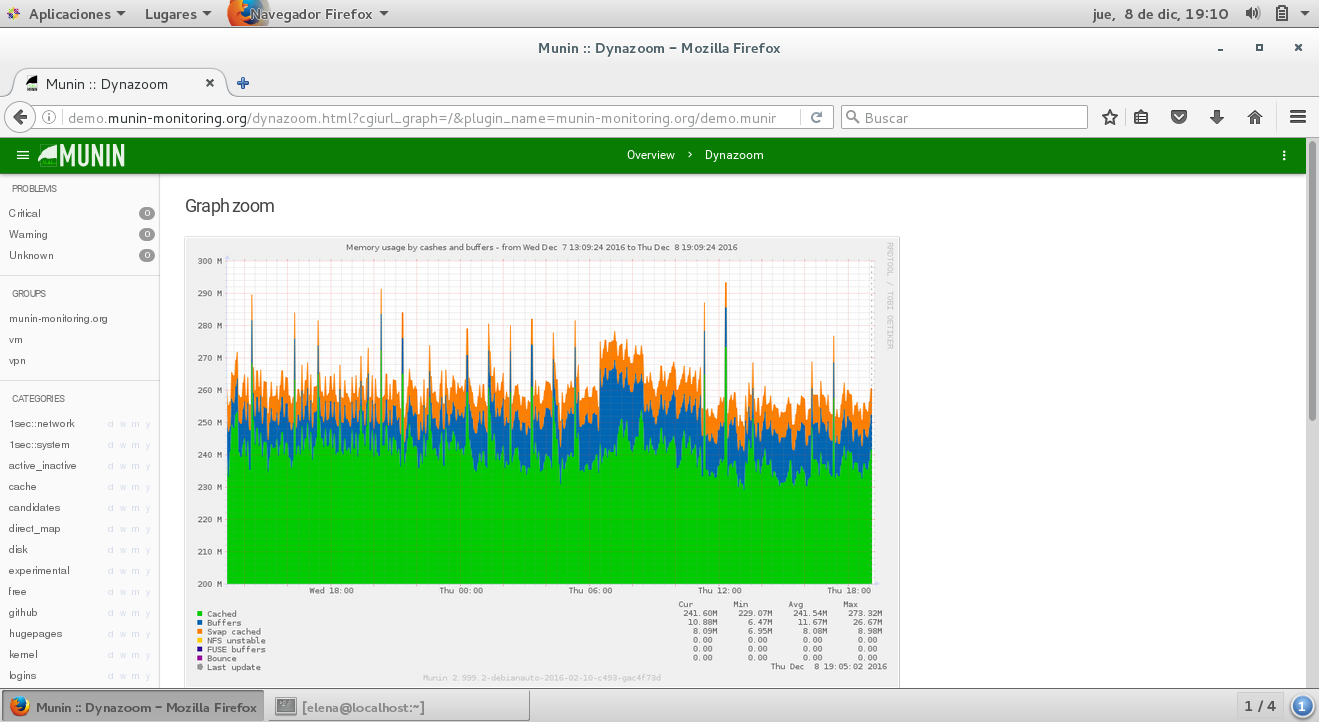
\includegraphics[width=14.7cm]{./img/ejercicio6_2.png} 	
	\caption{Demo munin, monitorización de la caché.} \label{fig:ejercicio6_2}
\end{figure}

\begin{figure}[H] 
	\centering
	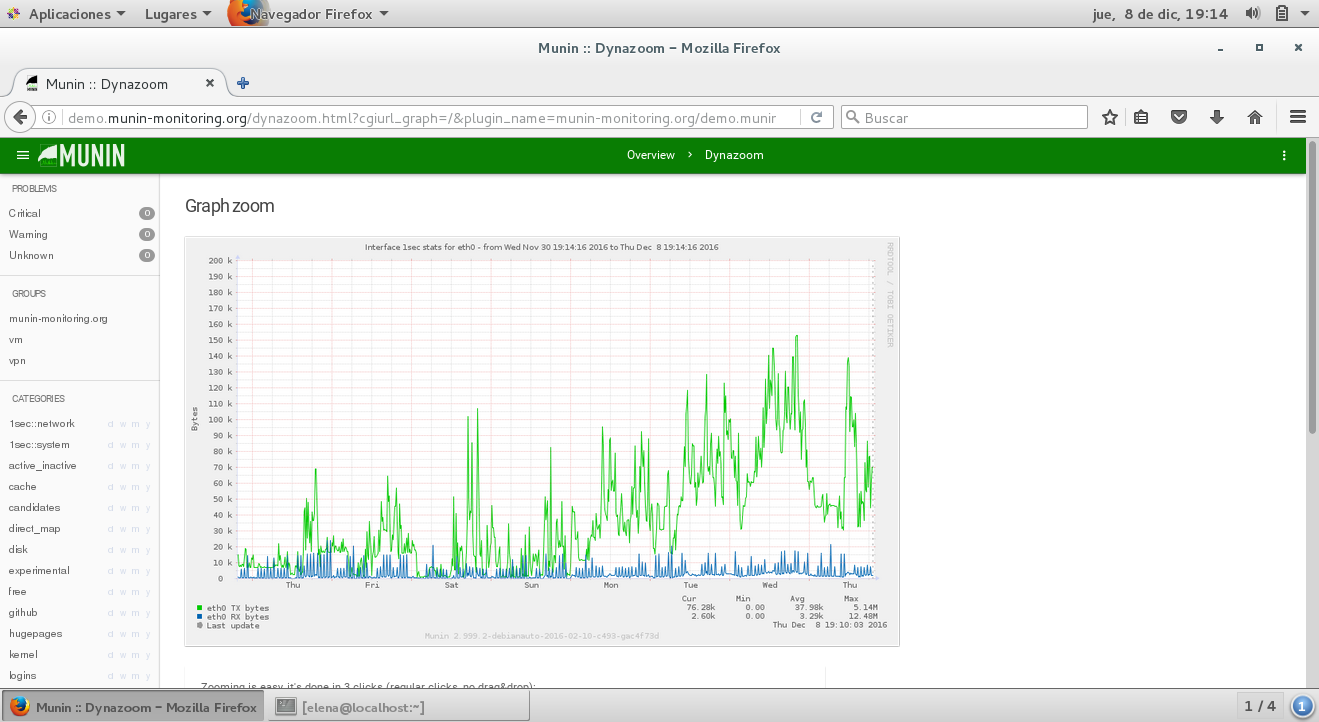
\includegraphics[width=14.7cm]{./img/ejercicio6_3.png} 	
	\caption{Demo munin, monitorización de la red.} \label{fig:ejercicio6_3}
\end{figure}

\begin{figure}[H] 
	\centering
	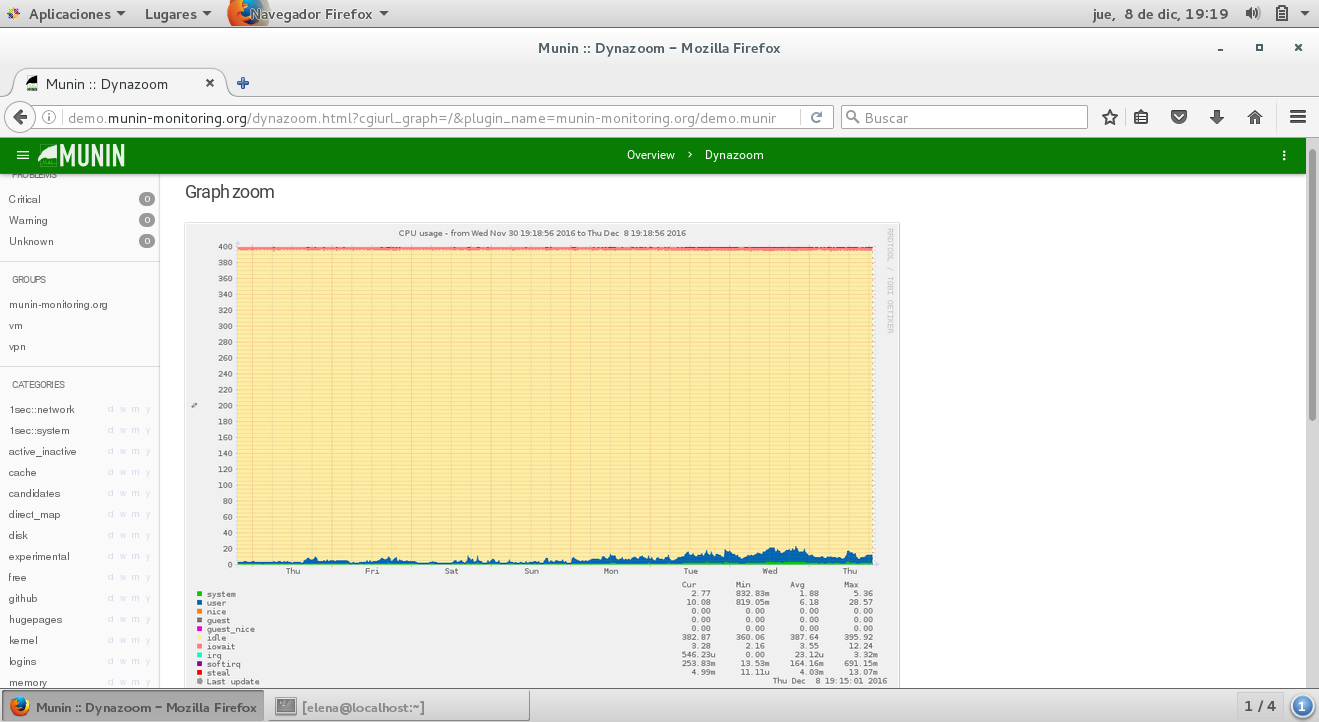
\includegraphics[width=14.7cm]{./img/ejercicio6_4.png} 	
	\caption{Demo munin, monitorización del uso de la CPU.} \label{fig:ejercicio6_4}
\end{figure}



%----------------------------------------------------------------------------------------
%  Cuestión opcional 2
%----------------------------------------------------------------------------------------

%\section{Cuestión opcional 2:}

%\subsection{Instale Nagios en su sistema (el que prefiera) documentando el proceso y muestre el resultado de la monitorización de su sistema comentando qué aparece.}


%----------------------------------------------------------------------------------------
%  Cuestión opcional 4
%----------------------------------------------------------------------------------------

\section{Cuestión opcional 4:}

\subsection{Pruebe a instalar este monitor en alguno de sus tres sistemas. Realice capturas de pantalla del proceso de instalación y comente capturas de pantalla del programa en ejecución.}

Para instalar ZABBIX utilizamos la documentación oficial \cite{zabbix}. Lo primero que debemos hacer es instalar el repositorio y posteriormente instalamos el server con mysql tal como se muestra en la figura \ref{fig:opcional4_1}. Creamos la base de datos tal y como se muestra en la figura \ref{fig:opcional4_2} e inicializamos el servicio.

Una vez hecho esto editamos el archivo de configuración \texttt{/etc/zabbix/zabbix\_server.conf} con la líneas: \\
DBHost=localhost\\
DBName=zabbix\\
DBUser=zabbix\\
DBPassword=zabbix\\

Una vez configurado reiniciamos los servicios, y desde el navegador ya se puede acceder a zabbix tal y como se muestra en la figura \ref{fig:opcional4_3}. La pantalla principal se ve en la figura \ref{fig:opcional4_4}, ademas podemos crear monitores como se muestra en las figuras \ref{fig:opcional4_5} y \ref{fig:opcional4_6}.

\begin{figure}[H] 
	\centering
	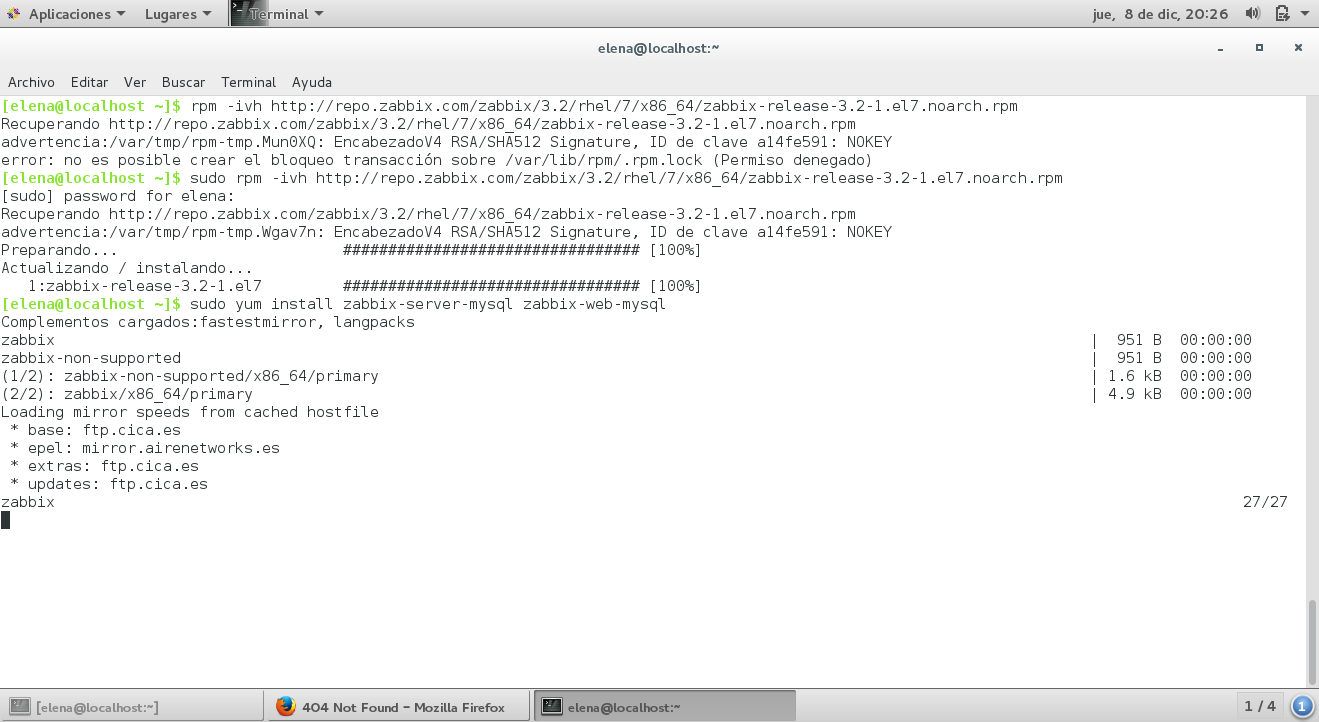
\includegraphics[width=14.7cm]{./img/opcional4_1.png} 	
	\caption{CentOS, instalación de zabbix.} \label{fig:opcional4_1}
\end{figure}

\begin{figure}[H] 
	\centering
	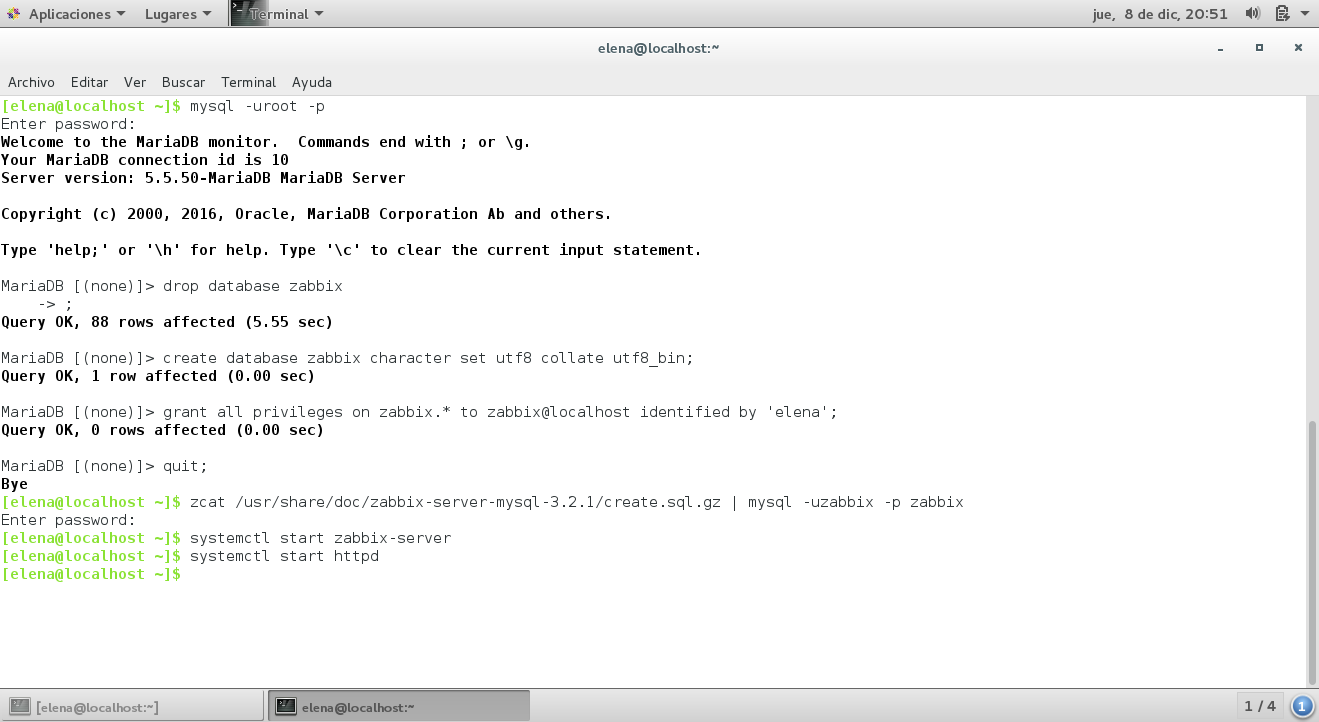
\includegraphics[width=14.7cm]{./img/opcional4_2.png} 	
	\caption{CentOS, configuración de zabbix.} \label{fig:opcional4_2}
\end{figure}

\begin{figure}[H] 
	\centering
	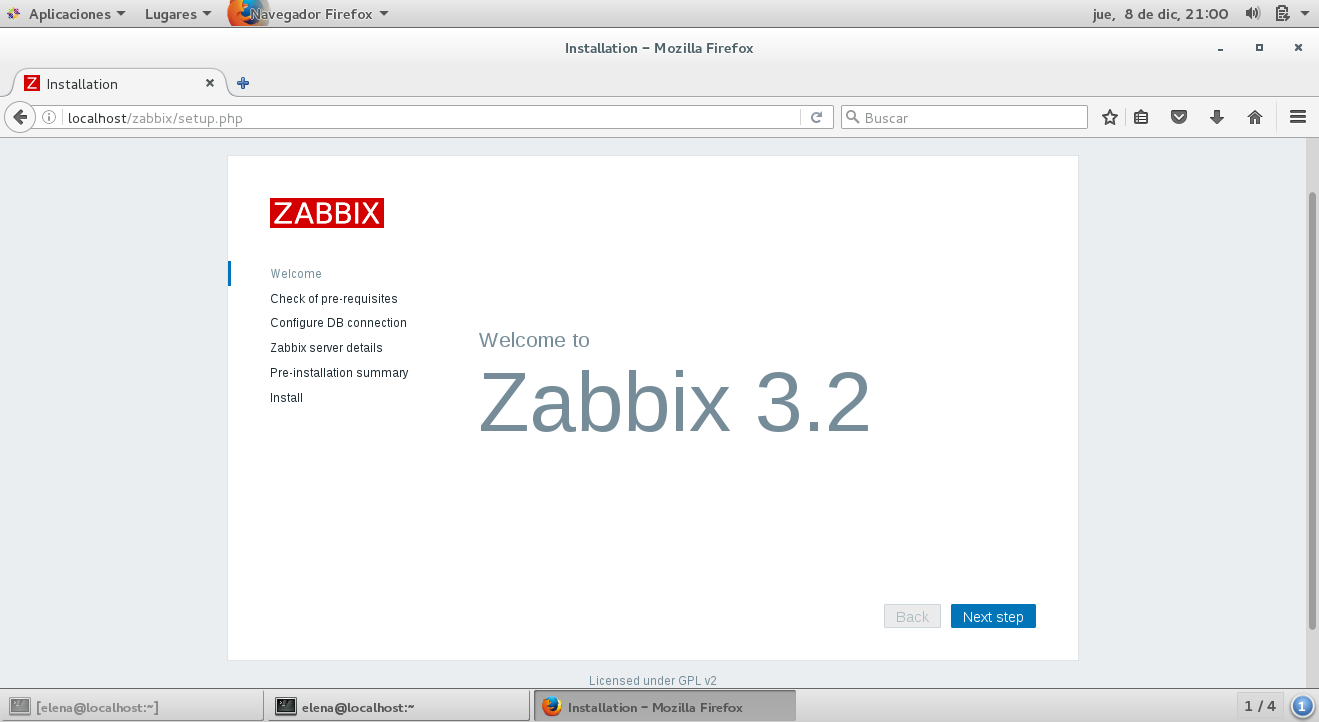
\includegraphics[width=14.7cm]{./img/opcional4_3.png} 	
	\caption{CentOS, zabbix.} \label{fig:opcional4_3}
\end{figure}

\begin{figure}[H] 
	\centering
	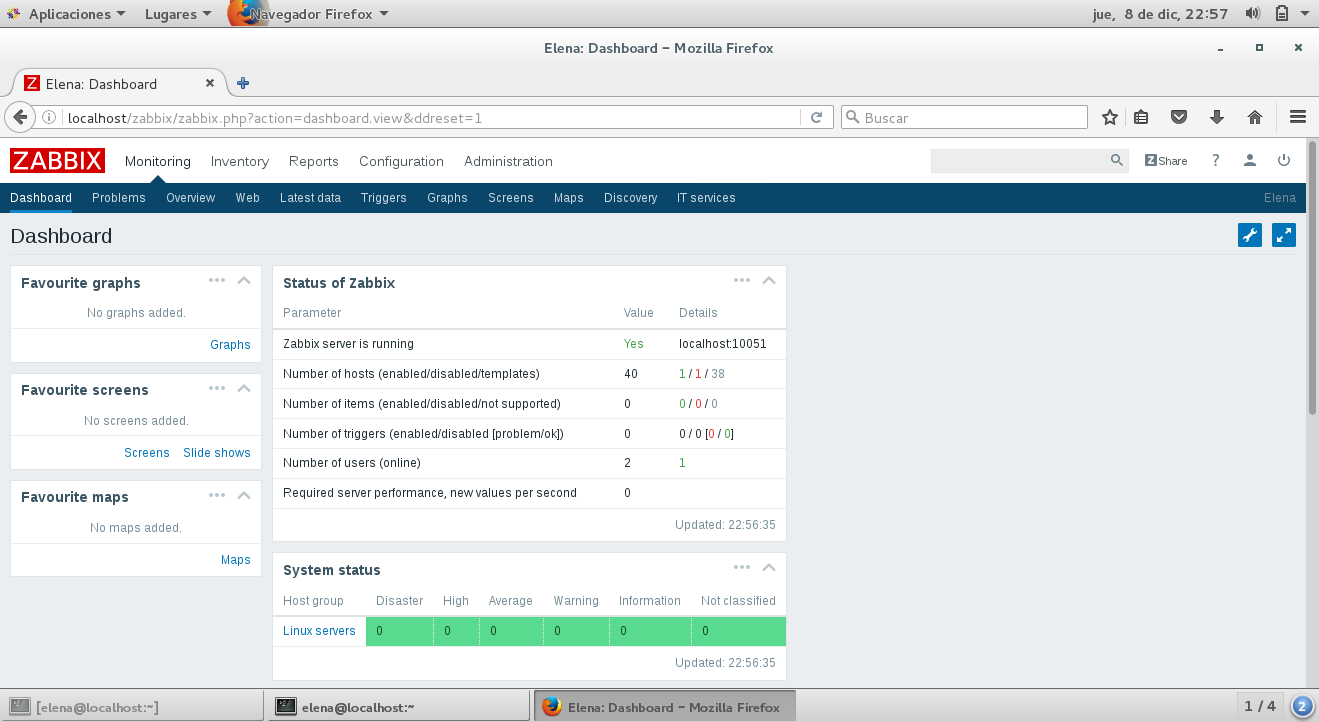
\includegraphics[width=14.7cm]{./img/opcional4_4.png} 	
	\caption{CentOS, zabbix.} \label{fig:opcional4_4}
\end{figure}

\begin{figure}[H] 
	\centering
	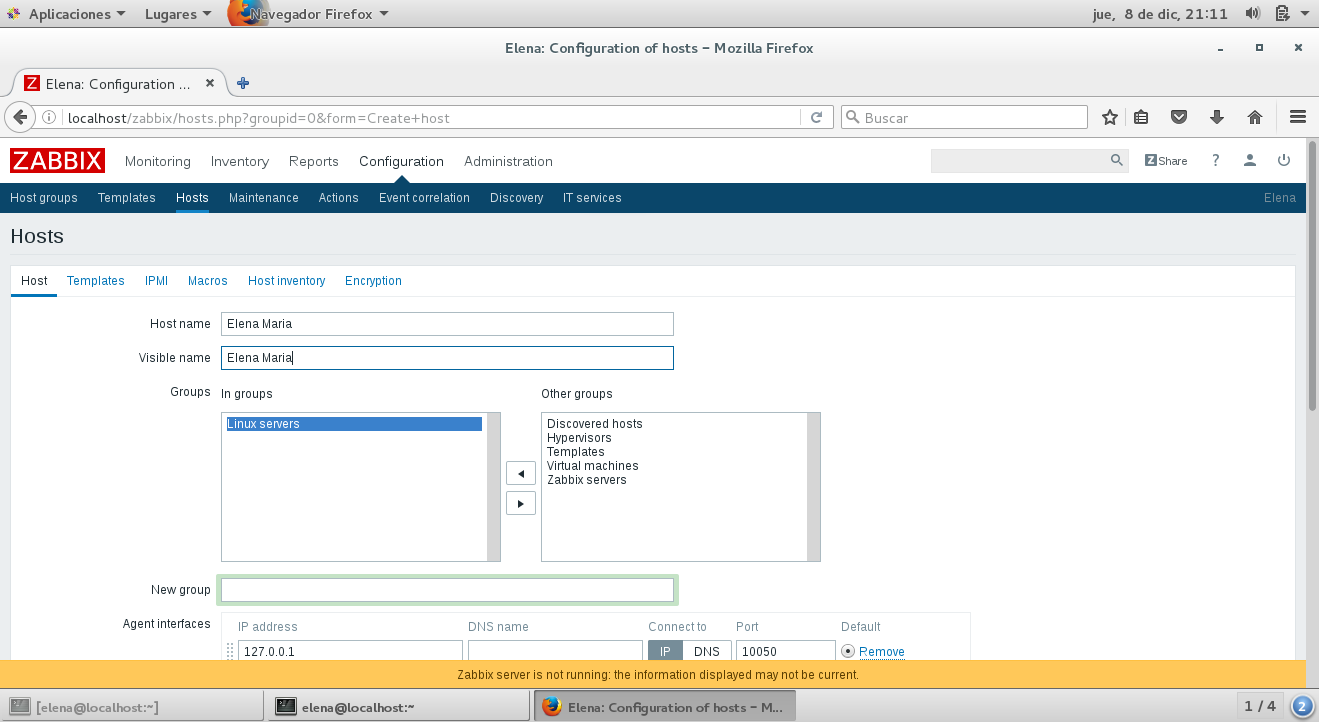
\includegraphics[width=14.7cm]{./img/opcional4_5.png} 	
	\caption{CentOS, zabbix.} \label{fig:opcional4_5}
\end{figure}

\begin{figure}[H] 
	\centering
	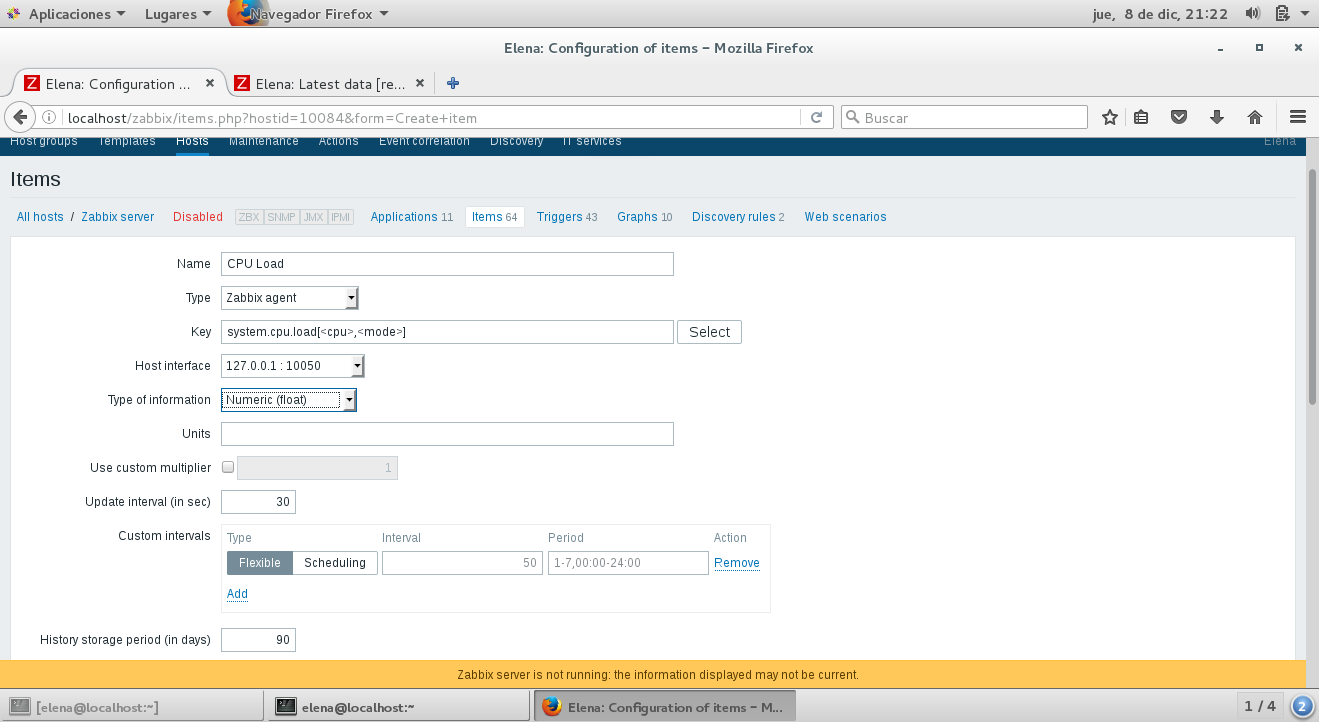
\includegraphics[width=14.7cm]{./img/opcional4_6.png} 	
	\caption{CentOS, zabbix.} \label{fig:opcional4_6}
\end{figure}


%----------------------------------------------------------------------------------------
%  Cuestión opcional 5
%----------------------------------------------------------------------------------------

%\section{Cuestión opcional 5:}

%\subsection{Pruebe a instalar este monitor en alguno de sus tres sistemas. Realice capturas de pantalla del proceso de instalación y comente capturas de pantalla del programa en ejecución.}


%----------------------------------------------------------------------------------------
%  Cuestión opcional 6
%----------------------------------------------------------------------------------------

%\section{Cuestión opcional 6:}

%\subsection{Instale el monitor. Muestre y comente algunas capturas de pantalla.}


%----------------------------------------------------------------------------------------
%  Cuestión 7
%----------------------------------------------------------------------------------------

\section{Cuestión 7:}

\subsection{Escriba un breve resumen sobre alguno de los artículos donde se muestra el uso de strace o busque otro y coméntelo.}

El artículo que voy a resumir es el de Chad Fowler, titulado ``The Magic of strace'' \cite{straceArticulo}.\\

En el artículo cuenta como arregló un problema que tenía que ver con los archivos que no eran adecuadamente accesibles en la base de datos del servidor de Lotus Domino. Para ello utilizó \texttt{strace}. \\

\texttt{Strace} es una herramienta de línea de comandos que permite monitorizar las llamadas al sistema usadas por un programa y todas las señales que éste recibe. En el artículo muestra un ejemplo simple de la utilización de \texttt{strace} en un programa en C el cuál simplemente imprime ``hi''. \texttt{Strace} hace que sea fácil mirar el funcionamiento interno de un proceso ya en ejecución, con la opción ``\texttt{-o}',' \texttt{strace} envía su salida a un archivo log.\\

En el artículo se explican las líneas principales de salida al utilizar \texttt{strace}, que significan y como podemos buscar ayuda sobre su utilización. Se explica cómo utilizando la combinación de \texttt{strace}, \texttt{lsof} y las páginas del \texttt{man} del sistema se pueden entender lo que un determinado programa está haciendo y así poder detectar errores.




%----------------------------------------------------------------------------------------
%  Cuestión 8
%----------------------------------------------------------------------------------------

\section{Cuestión 8:}

\subsection{Escriba un script en Python o PHP y analice su comportamiento usando el profiler presentado.}

En la figura \ref{fig:ejercicio8_1} se muestra el script en Python que voy a utilizar para analizar su comportamiento utilizando el profiler. En la figura \ref{fig:ejercicio8_2} se muestra la salida del profiler, para ello he utilzado el comando \texttt{python -m cProfiler P3ejercicio8.py}.

Ahora vamos a analizar la salida utilizando la ayuda de la documentación \cite{pythonProfiler}. Como podemos observar hay una llamada al script, esta llamada ha tardado 0,006 segundos, tanto excluyendo las llamadas a subfunciones (\texttt{tottime}) como incluyéndolas (\texttt{cumtime}).

\begin{figure}[H] 
	\centering
	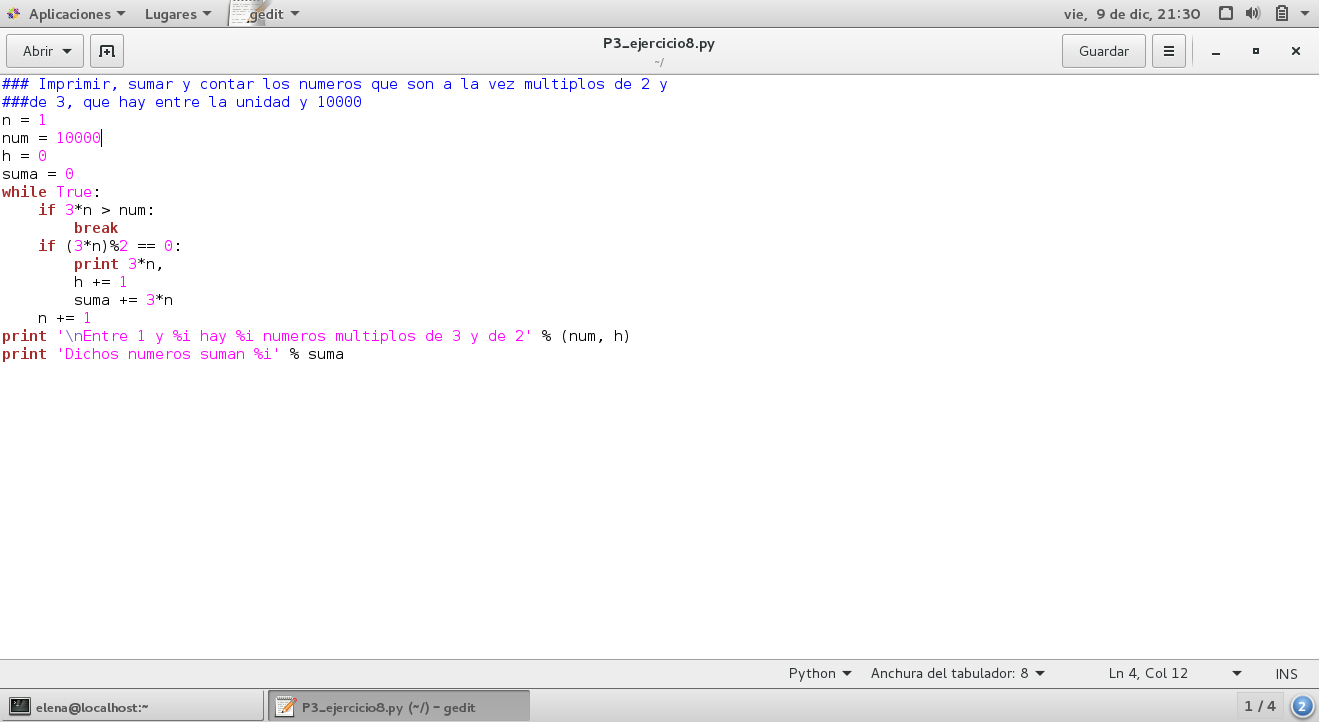
\includegraphics[width=14.7cm]{./img/ejercicio8_1.png} 	
	\caption{CentOS, código en python.} \label{fig:ejercicio8_1}
\end{figure}

\begin{figure}[H] 
	\centering
	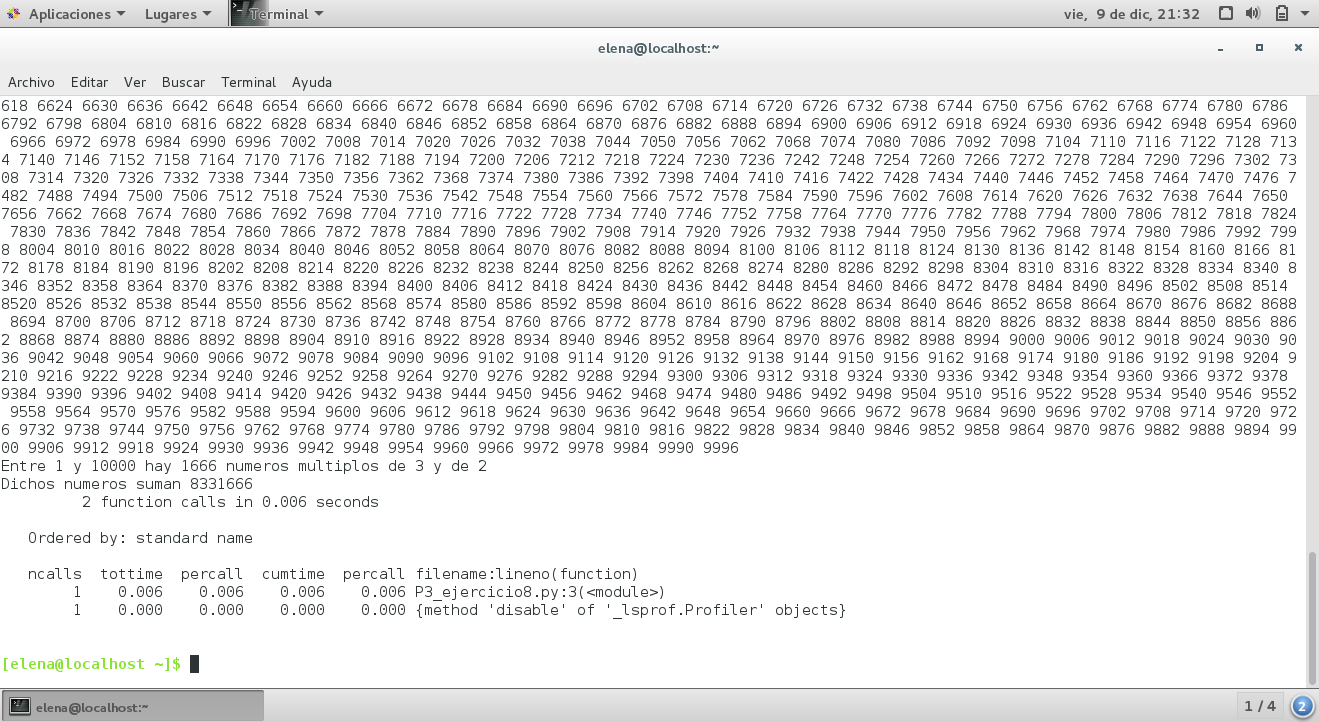
\includegraphics[width=14.7cm]{./img/ejercicio8_2.png} 	
	\caption{CentOS, profiling de un script en pyhton.} \label{fig:ejercicio8_2}
\end{figure}

%----------------------------------------------------------------------------------------
%  CCuestión opcional 10
%----------------------------------------------------------------------------------------

%\section{Cuestión opcional 10:}

%\subsection{Escriba un script en PowerShell y analice su comportamiento usando el %profiler presentado.}

%----------------------------------------------------------------------------------------
%  Cuestión 9
%----------------------------------------------------------------------------------------

\section{Cuestión 9:}

\subsection{Acceda a la consola mysql (o a través de phpMyAdmin) y muestre el resultado de mostrar el ”profile” de una consulta (la creación de la BD y la consulta la puede hacer libremente).}

Nos conectamos a la base de datos ``Prueba'' de MySQL, miramos si está activado el profiling, con el comando \texttt{SELECT @@profiling;},  y de no ser así lo activamos con \texttt{SET profiling = 1;}. Borramos y creamos una tabla para que el profiling pueda evaluar estas dos consultas. Todo esto se muestra en la figura \ref{fig:ejercicio9_1}.

Mostramos los profiling y los datos del profile tal y como se muestra en la figura \ref{fig:ejercicio9_2}. Mostramos los resultados del profiling de la primera consulta correspondiente al DROP, con el comando \texttt{SHOW PROFILE FOR QUERY 1;} (figura \ref{fig:ejercicio9_3}). Para la segunda consulta, correspondiente al CREATE, mostramos el profiling de la CPU con el comando \texttt{SHOW PROFILE CPU FOR QUERY 2;} como se muestra en la figura \ref{fig:ejercicio9_4}.

\begin{figure}[H] 
	\centering
	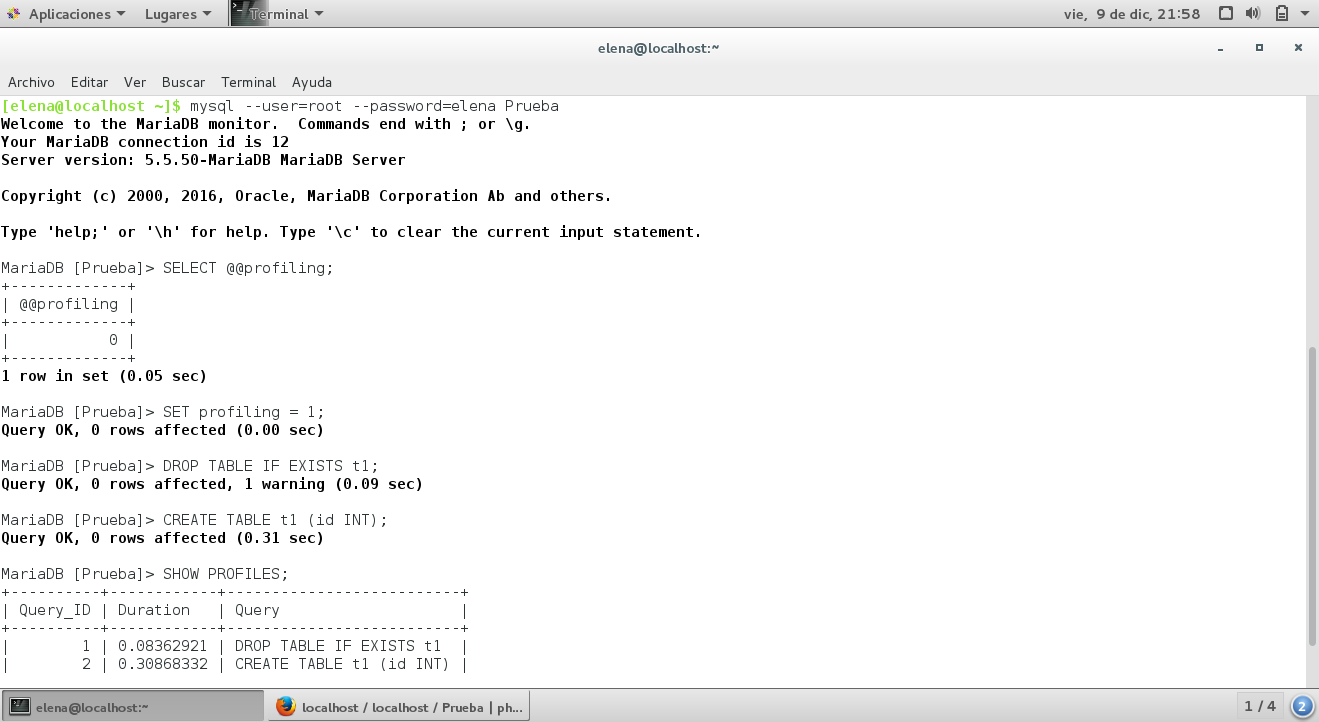
\includegraphics[width=14.7cm]{./img/ejercicio9_1.png} 	
	\caption{CentOS, profiling MySQL.} \label{fig:ejercicio9_1}
\end{figure}

\begin{figure}[H] 
	\centering
	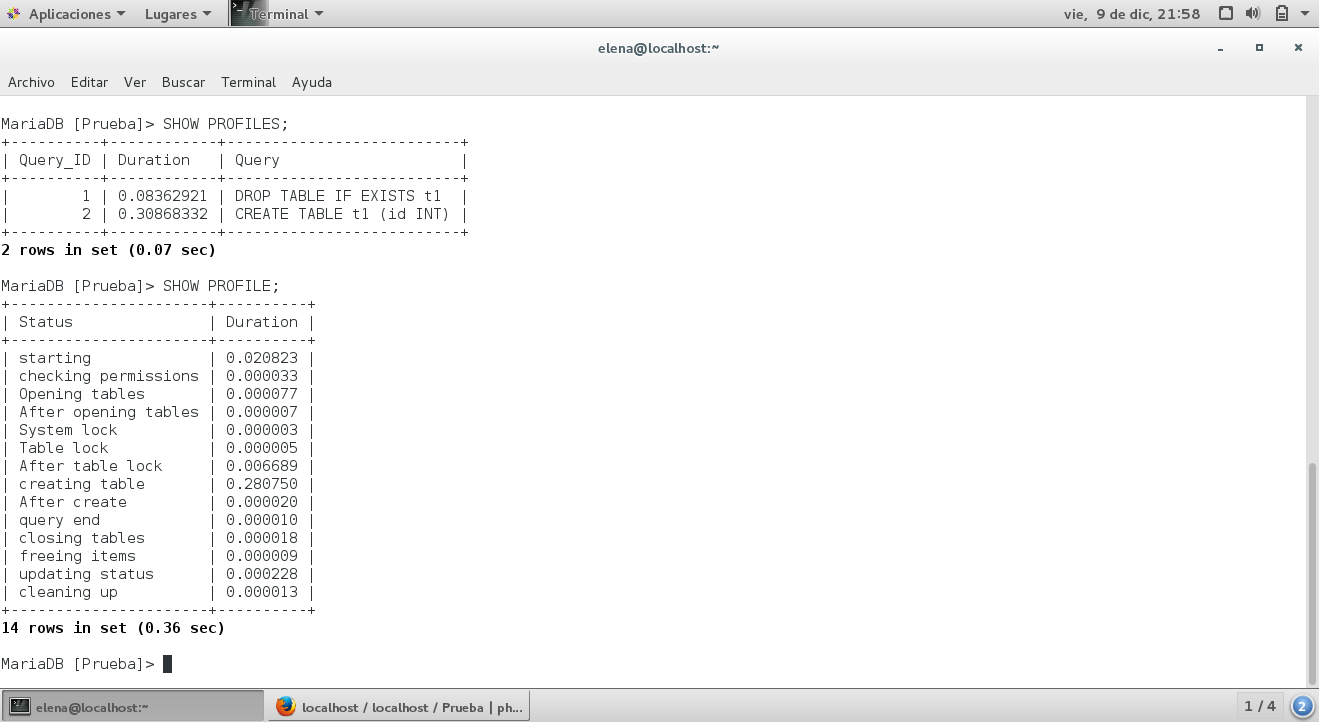
\includegraphics[width=14.7cm]{./img/ejercicio9_2.png} 	
	\caption{CentOS, profiling MySQL.} \label{fig:ejercicio9_2}
\end{figure}

\begin{figure}[H] 
	\centering
	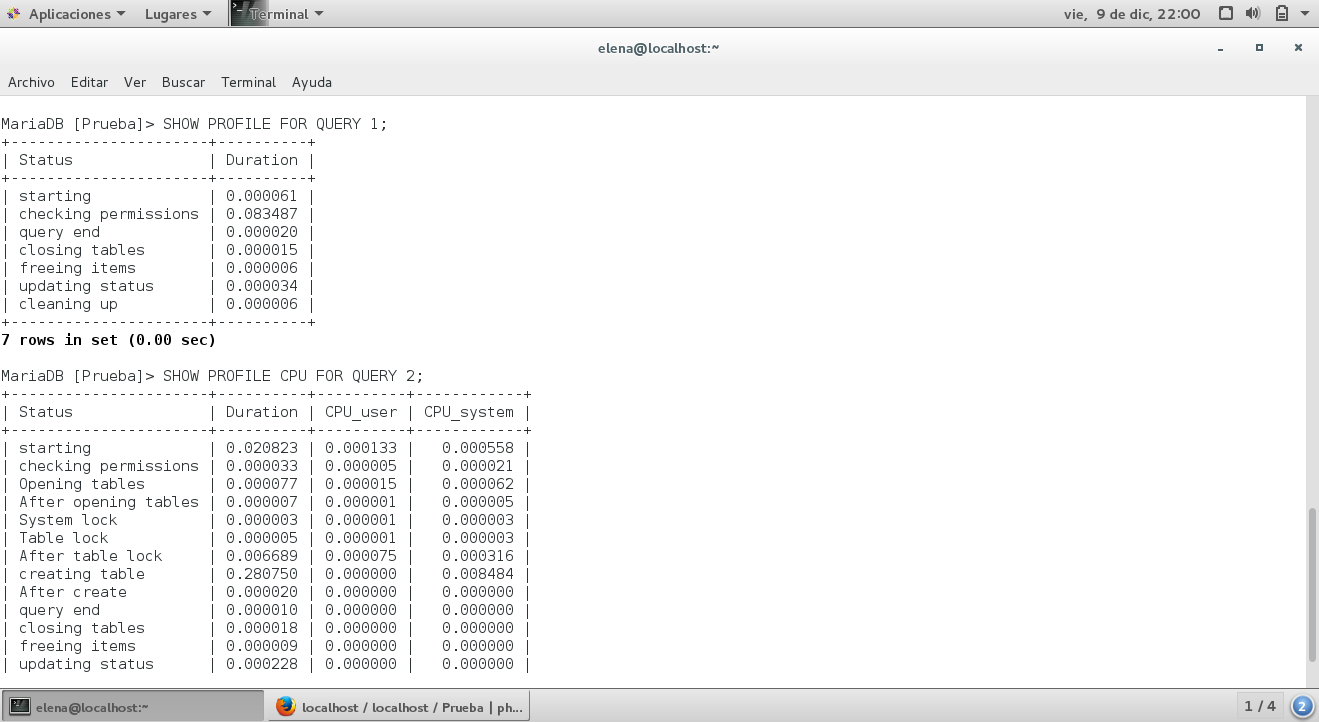
\includegraphics[width=14.7cm]{./img/ejercicio9_3.png} 	
	\caption{CentOS, profiling MySQL.} \label{fig:ejercicio9_3}
\end{figure}

\begin{figure}[H] 
	\centering
	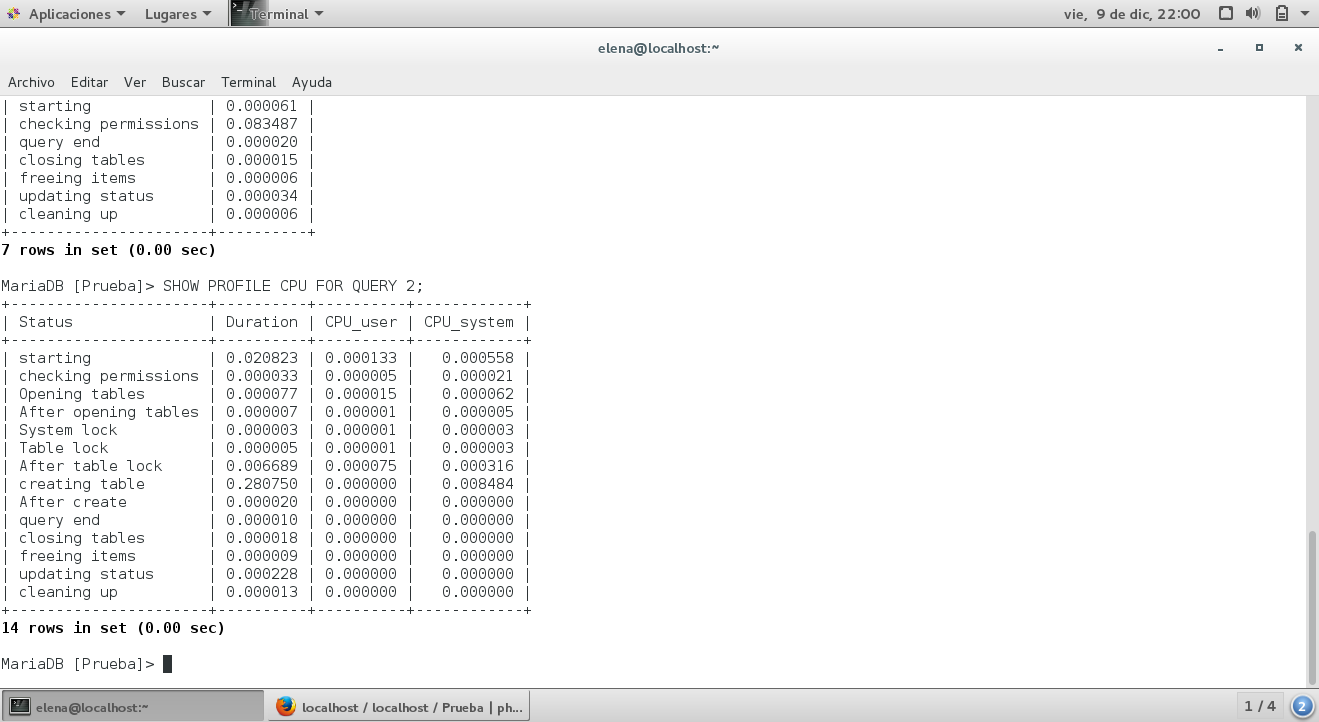
\includegraphics[width=14.7cm]{./img/ejercicio9_4.png} 	
	\caption{CentOS, profiling MySQL.} \label{fig:ejercicio9_4}
\end{figure}


%----------------------------------------------------------------------------------------
%  Cuestión opcional 11
%----------------------------------------------------------------------------------------

%\section{Cuestión opcional 11:}

%\subsection{Al igual que ha realizado el “profiling” con MySQL, realice lo mismo %con MongoDB y compare los resultados (use la misma información y la misma %consulta, hay traductores de consultas SQL a Mongo).}


%----------------------------------------------------------------------------------------
%  Extra
%----------------------------------------------------------------------------------------

\section{Tareas extra:}

\subsection{Monitorización del Hardware en Linux}

He probado los dos monitorizadores de Hardware que se indican en el guión. Como se muestra en la figura \ref{fig:extra_1_1} he instalado \texttt{hddtemp} y he comprobado la temperatura del disco sda, que es de 33º. También he instalado la GUI \texttt{xsensor} de \texttt{lm-sensor} como se muestra en la figura \ref{fig:extra_1_2} y probado su funcionamiento como se muestra en las figuras (\ref{fig:extra_1_3}, \ref{fig:extra_1_4} y \ref{fig:extra_1_5} ).

\begin{figure}[H] 
	\centering
	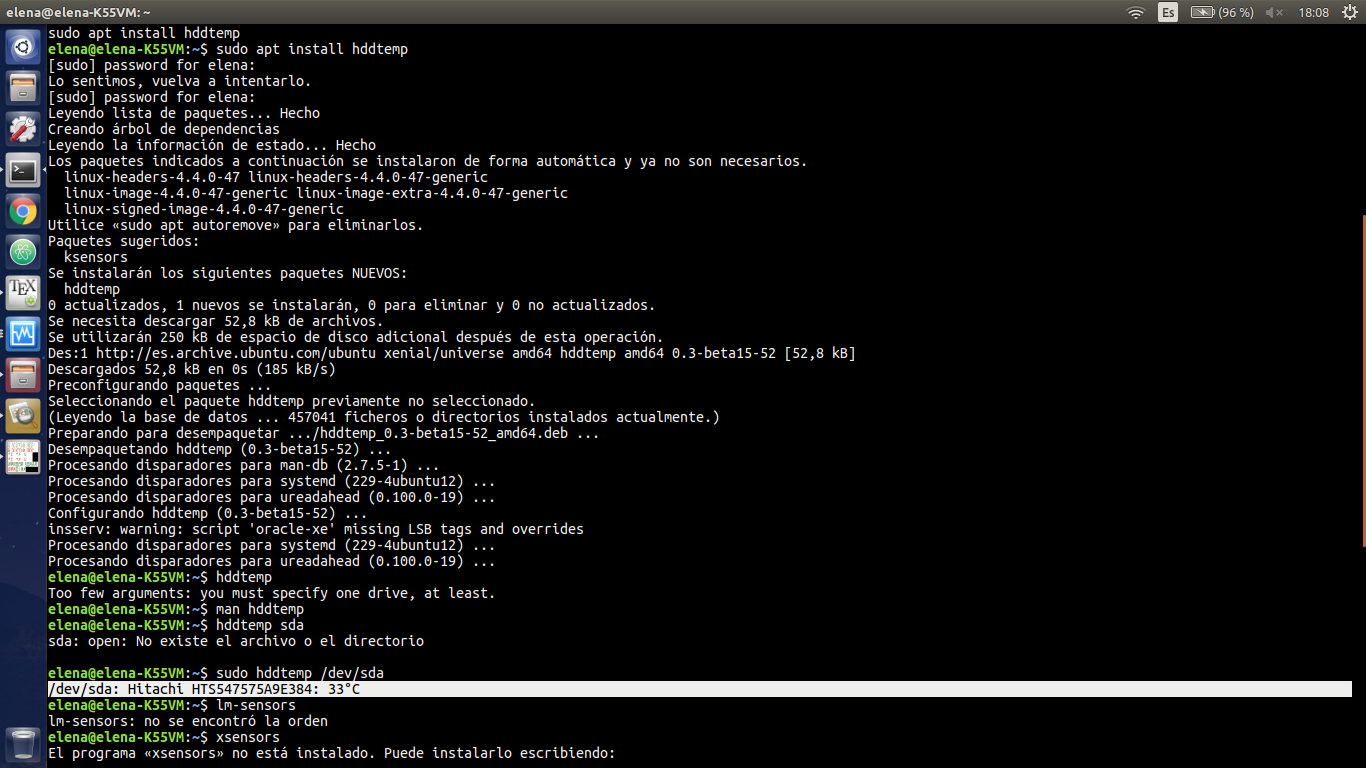
\includegraphics[width=14.7cm]{./img/extra_1_1.png} 	
	\caption{Ubuntu, instalación y ejecución de hddtemp.} \label{fig:extra_1_1}
\end{figure}

\begin{figure}[H] 
	\centering
	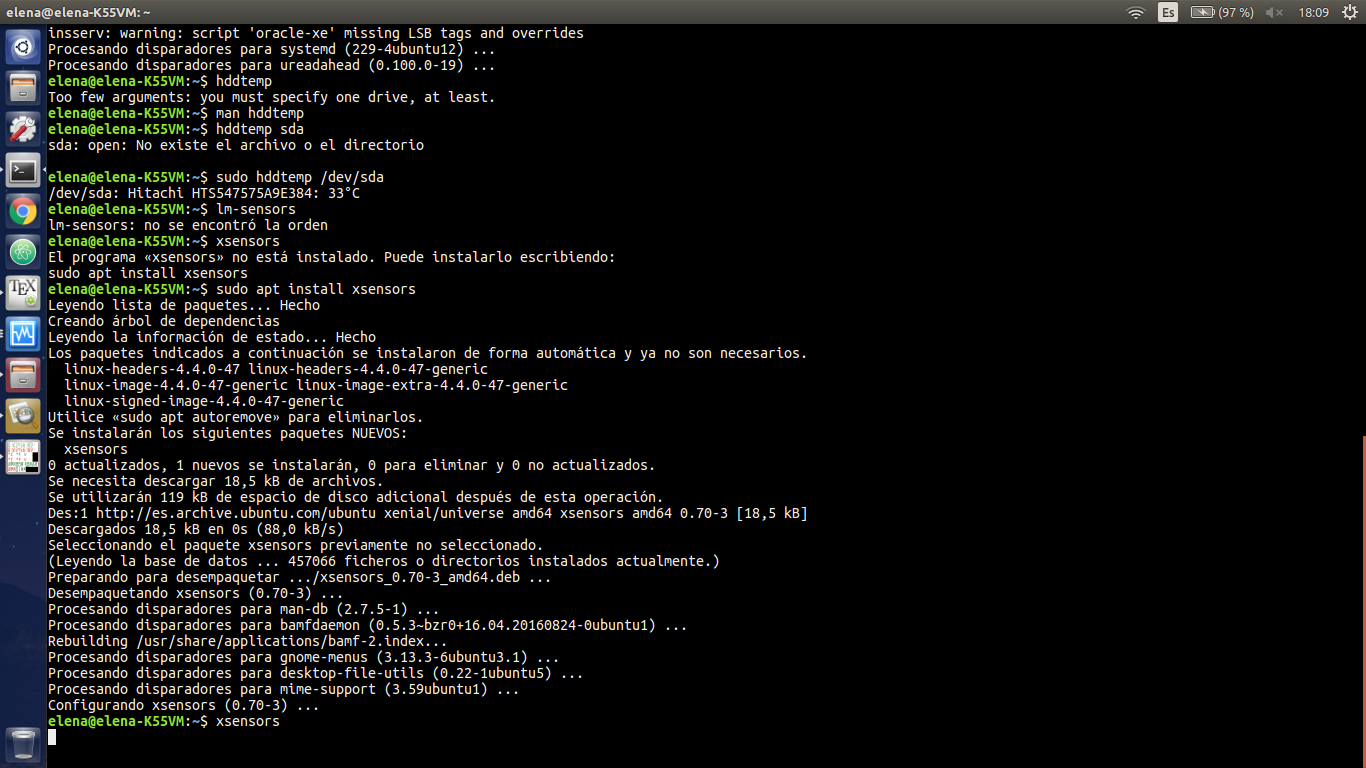
\includegraphics[width=14.7cm]{./img/extra_1_2.png} 	
	\caption{Ubuntu, instalación de lm-sensor con GUI xsensor.} \label{fig:extra_1_2}
\end{figure}

\begin{figure}[H] 
	\centering
	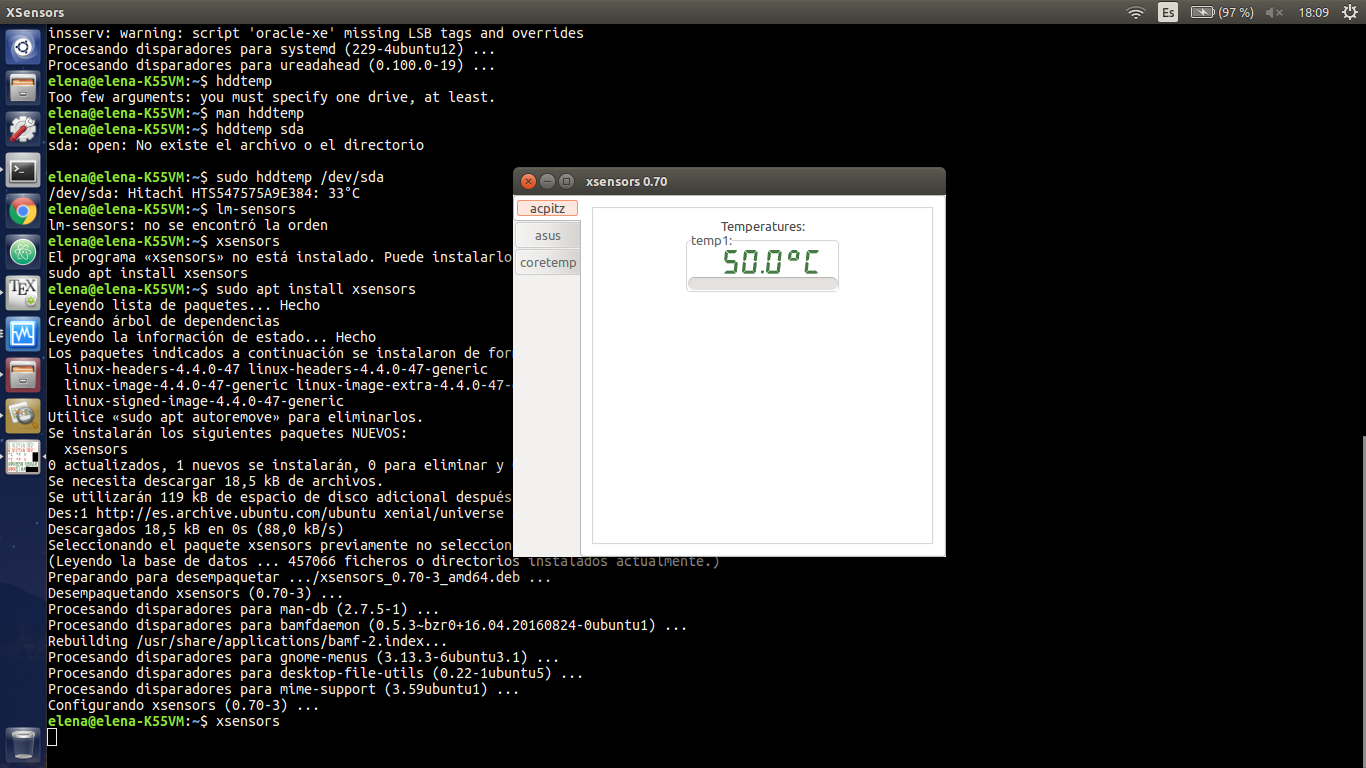
\includegraphics[width=14.7cm]{./img/extra_1_3.png} 	
	\caption{Ubuntu, xsensor, temperatura general.} \label{fig:extra_1_3}
\end{figure}

\begin{figure}[H] 
	\centering
	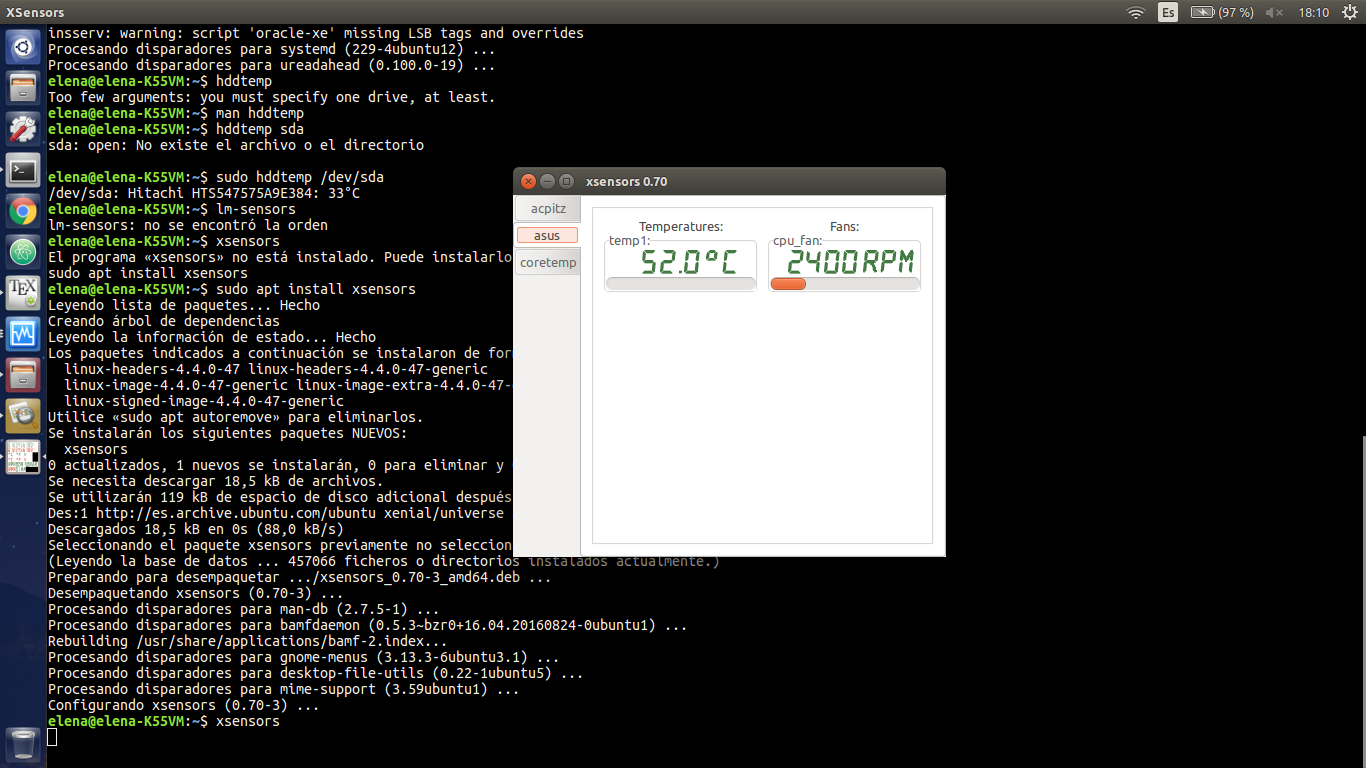
\includegraphics[width=14.7cm]{./img/extra_1_4.png} 	
	\caption{Ubuntu, xsensor, asus.} \label{fig:extra_1_4}
\end{figure}

\begin{figure}[H] 
	\centering
	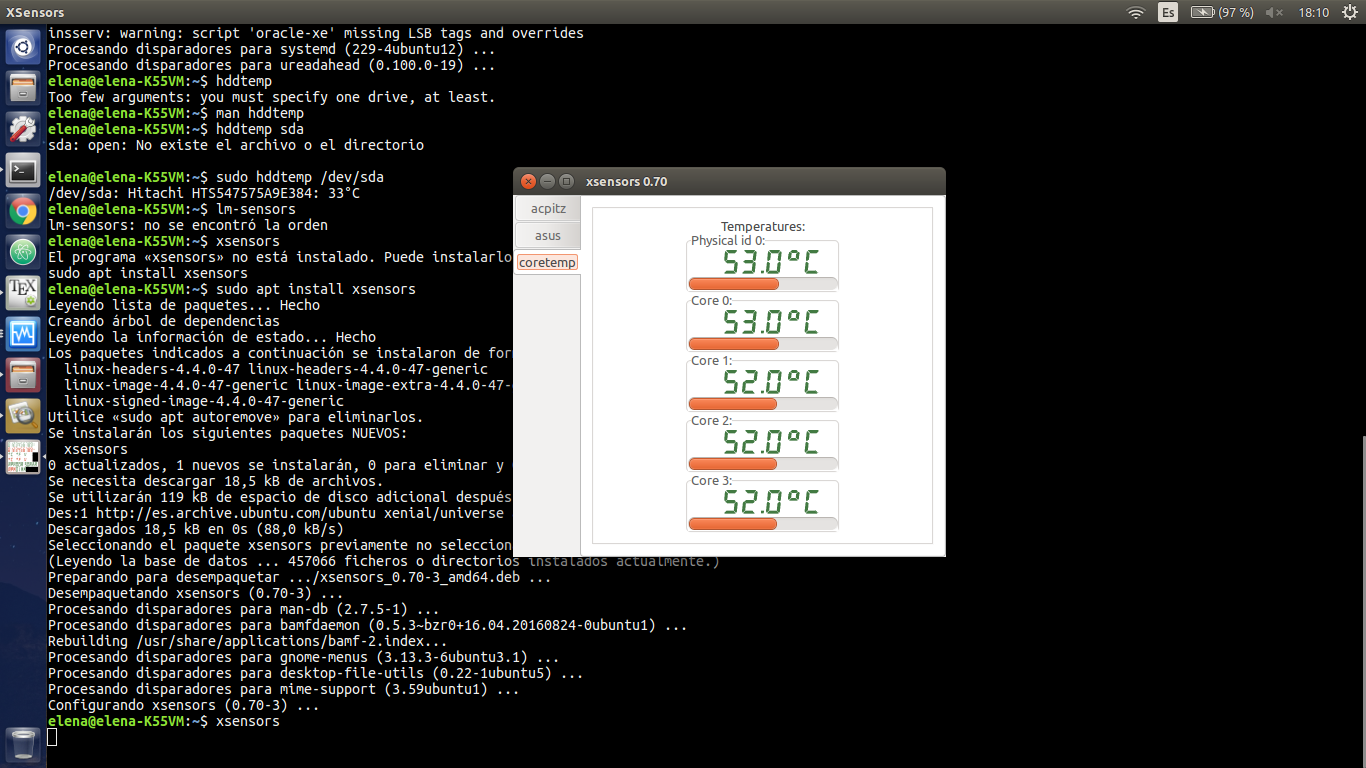
\includegraphics[width=14.7cm]{./img/extra_1_5.png} 	
	\caption{Ubuntu, xsensor, procesador.} \label{fig:extra_1_5}
\end{figure}


%------------------------------------------------

\bibliography{citas} %archivo citas.bib que contiene las entradas 
\bibliographystyle{plain} % hay varias formas de citar

\end{document}
